%!TEX program = xelatex
% !BIB program = biber

\documentclass[AutoFakeBold]{hutbthesis}

\usepackage{calc}
\usepackage{float}
\usepackage{longtable}
\usepackage{booktabs}
\usepackage{array}
\usepackage{tabularx}
\usepackage{caption}
\usepackage{xcolor}
\usepackage{listings}
\usepackage{amsmath}
\usepackage{chngcntr}
\usepackage{xeCJKfntef}

\counterwithin{figure}{chapter}
\counterwithin{table}{chapter}
\numberwithin{equation}{chapter}
\renewcommand{\thefigure}{\thechapter-\arabic{figure}}
\renewcommand{\thetable}{\thechapter-\arabic{table}}
\renewcommand{\theequation}{\thechapter-\arabic{equation}}
\captionsetup[figure]{name=图,labelsep=space,font=small,skip=6pt}
\captionsetup[table]{name=表,labelsep=space,font=small,skip=6pt}

\definecolor{codebg}{RGB}{248,248,248}
\definecolor{codekw}{RGB}{0,92,175}
\definecolor{codestr}{RGB}{163,21,21}
\definecolor{codecom}{RGB}{0,128,0}
\renewcommand{\lstlistingname}{代码}
\lstdefinestyle{hutbcode}{%
  backgroundcolor=\color{codebg},
  basicstyle=\ttfamily\small,
  keywordstyle=\color{codekw}\bfseries,
  stringstyle=\color{codestr},
  commentstyle=\color{codecom}\itshape,
  numbers=left,
  numberstyle=\scriptsize\color{gray},
  stepnumber=1,
  numbersep=8pt,
  frame=single,
  rulecolor=\color{gray!50},
  breaklines=true,
  columns=fullflexible,
  keepspaces=true,
  showstringspaces=false,
  tabsize=2,
  captionpos=b
}
\lstset{style=hutbcode}
\providecommand{\tightlist}{\setlength{\itemsep}{0pt}\setlength{\parskip}{0pt}}
\newcommand{\linkcite}[1]{\textsuperscript{\hyperlink{ref:#1}{[#1]}}}
\IfFontExistsTF{Noto Serif CJK SC}{%
  \setCJKmainfont{Noto Serif CJK SC}[BoldFont=Noto Serif CJK SC Bold]
  \setCJKsansfont{Noto Sans CJK SC}[BoldFont=Noto Sans CJK SC Bold]
}{}
\graphicspath{{images/}}

%!TEX root = ../hutbthesis_main.tex

% 文章信息
\titlecn{基于人机交互强化的固定翼飞行器着陆控制系统}
\titleen{Landing Control System of Fixed-Wing Aircraft Enhanced by Human-Machine Interaction}

\author{马嘉骏}
\subsupervisor{}
\studentid{2209040025}
\priormajor{机器人工程}
\myclass{机器人工程2201}
\supervisor{王海东讲师}
\department{智能机器人学院}
\thesisdate{year=2026, month=5}

\clcnumber{TP391}
\schoolcode{10554}
\udc{004.9}
\academiccategory{学术学位}


\begin{document}

\maketitle

\clearpage
\pagestyle{empty}
\pagenumbering{gobble}
%!TEX root = ../hutbthesis_main.tex

\begin{declarationzh}

本人郑重声明：所呈交的本科毕业设计《基于人机交互强化的固定翼飞行器着陆控制系统》是本人在指导老师的指导下，独立进行研究工作所取得的成果，成果不存在知识产权争议，除文中已经注明引用的内容外，本设计不含任何其他个人或集体已经发表或撰写过的作品成果。对设计的研究做出重要贡献的个人和集体均已在文中以明确方式标明。本人完全意识到本声明的法律结果由本人承担。

\vspace{30pt}
\begin{flushright}
作者签名：
\includegraphics[width=2.8cm]{images/image2.jpeg}\qquad\par
日\qquad 期：2026年5月25日\qquad
\end{flushright}

\end{declarationzh}

\clearpage
%!TEX root = ../hutbthesis_main.tex

\chapter*{湖南工商大学本科毕业设计\protect\\版权使用授权书}

本毕业设计《基于人机交互强化的固定翼飞行器着陆控制系统》是本人在校期间所完成学业的组成部分，是在学校教师的指导下完成的。因此，本人特授权学校可将本毕业设计的全部或部分内容编入有关书籍、数据库保存，可采用复制、印刷、网页制作等方式将设计文本和经过编辑、批注等处理的文本提供给读者查阅、参考，可向有关学术部门和国家有关教育主管部门呈送复印件和电子文档。本毕业设计无论做何种处理，必须尊重本人的著作权，署明本人姓名。

\vspace{80pt}
\noindent 论文作者（签字）：
\includegraphics[width=2.4cm]{images/image3.jpeg}\hfill 时间：2026年5月25日

\vspace{50pt}
\noindent 指导教师已阅（签字）：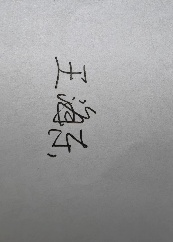
\includegraphics[angle=90,origin=c,width=2.6cm]{images/image4.jpeg}\hfill 时间：2026年5月25日

\clearpage
%!TEX root = ../hutbthesis_main.tex

% 设置中文摘要
\keywordscn{固定翼飞行器，着陆控制，人机交互强化}
\begin{abstractzh}

固定翼飞行器着陆阶段是飞行全过程中风险较高、控制要求较强的关键环节，易受到速度、下沉率、姿态偏差、侧偏误差及地形环境等因素影响。本文以基于人机交互强化的固定翼飞行器着陆控制系统为研究对象，围绕系统组成与需求分析、动力学模型建立、仿真平台实现、多工况结果分析以及交互强化策略设计等内容展开研究。首先，对着陆任务场景、关键参数及影响因素进行了分析；其次，建立了着陆阶段动力学模型和仿真模型，并完成基准工况校核；再次，通过平坦、起伏、山脊、谷地和阶跃等不同地形工况的仿真对比，分析了飞行器在着陆末段的离地高度、速度和姿态变化规律，识别出阶跃地形为典型不利工况；最后，提出了风险识别、状态提示、操纵辅助和约束保护相结合的人机交互强化策略。研究表明，该方法能够在一定程度上提高固定翼飞行器在复杂工况下的着陆安全性与稳定性，为后续控制系统优化提供参考。

\end{abstractzh}

\clearpage
%!TEX root = ../hutbthesis_main.tex

% 设置英文摘要
\keywordsen{Fixed-wing Aircraf; Landing Control; Human-Machine Interaction Enhancement}
\begin{abstracten}

The landing phase of a fixed-wing aircraft constitutes a critical stage
within the entire flight process---one characterized by elevated risk
and stringent control requirements---as it is susceptible to various
influencing factors such as velocity, sink rate, attitude deviations,
lateral drift errors, and terrain conditions. This paper focuses on a
fixed-wing aircraft landing control system enhanced through
human-machine interaction. The research encompasses a comprehensive
scope, including system architecture and requirements analysis, dynamic
modeling, simulation platform implementation, multi-scenario result
analysis, and the design of human-machine interaction enhancement
strategies. First, the landing mission scenarios, key parameters, and
influencing factors were thoroughly analyzed. Second, dynamic and
simulation models for the landing phase were established, followed by
the verification of a baseline operational scenario. Third, through
comparative simulations across diverse terrain conditions---including
flat, undulating, ridge, valley, and step-like profiles---the behavioral
patterns of the aircraft\textquotesingle s ground clearance, velocity,
and attitude during the final approach were analyzed; this analysis
identified the step-like terrain as a representative adverse scenario.
Finally, a human-machine interaction enhancement strategy was proposed
that integrates risk identification, status prompting, control
assistance, and constraint protection. The findings indicate that this
approach can, to a significant extent, enhance the safety and stability
of fixed-wing aircraft landings under complex operational conditions,
thereby providing a valuable reference for the subsequent optimization
of control systems.

\end{abstracten}


\frontmatter
\setcounter{page}{1}
\tableofcontents

\mainmatter
%!TEX root = ../hutbthesis_main.tex

\chapter{绪论}

\section{研究背景与研究意义}

固定翼飞行器着陆阶段是属于飞行全过程中里风险相对较高的环节之一。与跟巡航阶段相比较而言，着陆的时候飞行高度较低、，速度变化较快、，操纵时间较短，容极易受到侧风、低空湍流、地面效应以及、姿态扰动等因素影响的作用，进从而导致引发接地点偏差、下沉率过大、姿态超限和、滑跑偏移等问题。若要是控制不得当的话，不仅但会影响着陆质量，还可能对给飞行器结构安全和、后续运行造成带来不利影响。

随着固定翼飞行器特别是无人机，于巡检、测绘、侦察、运输等诸多领域被广泛运用，飞行任务所处的环境变得越来越复杂，这对着陆控制系统的安全性、稳定性、适应性，提出了更为严苛的要求。当前现有的着陆控制研究，主要聚焦于控制算法、轨迹跟踪、姿态调节等方面，虽说能够在一定程度上提高着陆精度，然而对于操纵者在着陆进程里的信息获取、风险判断、操作辅助，所给予的关注却相对欠缺。

在人机协同日益强化的背景状况下，把人机交互强化思想引入到固定翼飞行器着陆控制系统当中，借助状态提示、风险告警、操纵辅助、安全约束等多种方式，能够帮助操纵者更为精准地把握飞行状态，及时对操作予以修正，进而降低着陆风险。所以，对基于人机交互强化的固定翼飞行器着陆控制系统展开研究，具备颇为显著的现实意义。

从理论意义来讲，展开对于基于人机交互强化的固定翼飞行器着陆控制系统的研究，能够推动着陆控制研究从单一控制律设计朝着``控制层---交互层---保护层''协同设计方向延伸拓展，进而丰富固定翼飞行器着陆控制系统的研究内容，并且完善相关评价指标模式、设计方法。

从工程意义方面分析，此项研究可为固定翼飞行器在复杂工况时实现安全着陆提供更具操作性的系统方案，能为后续着陆控制仿真验证、模块化设计、工程应用给予参考。以人机交互强化作为切入点来研究固定翼飞行器着陆控制系统，具备较强的理论价值与实际应用价值。

\section{国内外研究现状}

外国对于固定翼飞行器着陆的研究重点放在起落架结构设计、低速着陆气动特性、缓冲系统动力学、控制辅助等领域。Elahi等人针对无人作战飞行器CFRP起落架展开设计与分析，觉得复合材料起落架能在保证承载能力的情况下达成轻量化，为着陆阶段结构安全设计给出了参照。

Lampropoulos等人针对低速无人机展开研究，聚焦于其在起飞、着陆、大气湍流状况下的机翼气动性能表现。他们发现低空区域存在的湍流、低速流场发生的变化，会对飞行器的升阻特性、姿态稳定性产生明显影响，进而对着陆控制精度造成影响。Dinc等人则对舰载无人机油气式起落架系统的动力学特性做了分析，探究出气体压缩、液体节流、结构非线性耦合作用对于缓冲响应与冲击载荷具有重要作用。Jinjin等人围绕无人机起落架缓冲器，从优化设计、试验验证这两方面展开研究，其结果显示对结构参数与阻尼特性进行合理优化，能够有效降低着陆冲击峰值，同时提高缓冲性能。

另外，Baek等人提出了基于输入信号变换的控制辅助系统，目的在于改善无人机目标跟踪与着陆的性能，这为把人机交互强化思想引入着陆控制系统给予了启发\linkcite{5}。从整体情况来看，国外的研究成果比较丰富，不过多数研究仍侧重于结构、缓冲或控制中的某一项内容，对于控制、交互与安全约束协同设计的系统性研究相对欠缺。

在国内，针对固定翼飞行器、无人机着陆展开的研究里，重点聚焦于起落架结构的优化工作、整体布局的分析工作、缓冲器性能的研究工作等多个方面。帅涛针对某一型号的起落架进行了设计、模态分析，明确指出起落架的固有频率、振型对于着陆冲击响应会产生非常重要的影响。周著学、于萍借助有限元分析方法针对小型航拍无人机的起落架进行了优化设计，阐述了合理调整结构、材料参数能够让应力分布得到改善并且提高承载能力。薛影、张超、吴星星剖析了无人机起落架布置对于起飞性能所造成的影响，显示出起落架的几何布局、安装位置与飞行性能存在着显著的耦合关系，而这对于着陆控制系统的总体设计同样具备参考价值。

罗杰等人针对某型无人机起落架放下阶段缓冲器的气液流动特性展开了研究，进而揭示出缓冲器内部气液流动变化对于阻尼性能、响应过程所产生的影响。蒲雅熙是从油气缓冲器气液两相阻尼特性着手，对不同工况下缓冲器阻尼变化规律予以分析，表明着陆速度与冲击条件会直接作用于缓冲器工作状态\linkcite{10}。

目前国内在起落架设计、有限元优化还有缓冲性能分析这些方面已经取得了一些成果。不过现有研究更多的是关注结构设计、缓冲机理，对于着陆阶段操纵者状态感知、风险提示、操作辅助与输入约束等人机交互强化问题关注不足。

整体看来，国内外研究已经给固定翼飞行器着陆控制奠定了不错的基础，特别是在起落架结构设计、低速气动特性、缓冲器动力学等方面取得了较多成果。然而现有研究大多是围绕结构、缓冲或者控制其中某一个方面进行的，针对``人机交互强化''的系统研究比较欠缺，特别是在复杂工况下怎样借助状态提示、风险告警、操纵辅助、输入约束来提高着陆安全性与稳定性，依旧缺少比较完整的研究框架。所以本文在已有研究的基础上引入人机交互强化思想，探究固定翼飞行器着陆控制系统的优化设计，具备一定的理论意义与实际价值。

\section{研究内容与技术路线}
\subsection{研究内容}
本文以固定翼飞行器着陆过程为研究对象，围绕人机交互强化的着陆控制系统开展研究。首先，对固定翼飞行器着陆任务场景、系统组成及关键影响因素进行分析，明确着陆过程中速度、高度、下沉率、姿态偏差等主要参数及其作用。其次，建立着陆阶段动力学模型和仿真模型，为后续分析不同工况下的着陆性能提供基础。再次，设计模型校核方法、性能评价指标和典型工况，通过仿真计算分析不同工况下系统响应变化规律，识别不利工况与较优工况。最后，结合仿真结果提出人机交互强化策略，重点从风险告警、状态提示、操纵辅助和约束控制等方面进行分析，并提出系统优化建议。
\subsection{技术路线}
本文围绕着``需求分析---模型建立---仿真验证---结果分析---策略优化''这一思路来进行研究工作。一开始，借助查阅相关文献，同时紧密结合课题任务要求，去剖析固定翼飞行器着陆阶段的主要风险、控制需求，进而确定研究内容和评价指标。接着，依据着陆过程的特点建立动力学模型与仿真模型，并完成主要参数的设定工作。然后，设计不同工况下的仿真方案，针对着陆过程里的速度、姿态、下沉率、偏差等指标展开计算与比较分析。最后，基于上述工作识别系统存在的问题，提出人机交互强化策略，并且对其工程可实现性予以讨论，从而形成论文的研究结论。

%!TEX root = ../hutbthesis_main.tex

\chapter{固定翼飞行器着陆控制系统组成与需求分析}

\section{固定翼飞行器着陆任务场景与系统组成}

固定翼飞行器着陆阶段在其整个飞行过程当中，属于风险最为集中且操纵要求颇高的阶段范畴。依据本文仿真平台的运行逻辑剖析可知，飞行器的着陆过程能够被划分成进近、拉平、接地区域、滑跑这四个阶段。进近阶段的主要任务是实现下滑轨迹的维持、速度的有效控制、跑道的精准对准，拉平阶段主要是降低下沉速率并且对俯仰姿态加以调整，让飞行器平稳地向地面靠近，接地区域着重关注接地高度、姿态、侧偏误差，滑跑阶段重点对接地后的方向保持与状态收敛展开分析。着陆后段飞行高度较低、修正时间比较短且对环境扰动比较敏感，所以此阶段既要求控制系统具备稳定可靠性，又要求操纵者能够及时把握关键状态的变化情况并做出正确的决策。

就系统组成而言，本研究的固定翼飞行器着陆控制系统主要涵盖感知层、控制层、人机交互层、安全保护层这四个部分。感知层的作用是收集离地高度、速度、下沉率、俯仰角、滚转角、航向角、侧偏量还有地形高程等状态信息，它是达成闭环控制的根本所在，控制层会按照飞行状态、目标约束，实时产生油门、升降舵、副翼、方向舵、襟翼指令，以此来实现纵向和侧向的修正，人机交互层负责把关键状态、风险提示、建议操纵信息反馈给操纵者，安全保护层会依据阈值判断是不是需要限幅、约束或者复飞。由此能够知道，着陆控制系统并非单纯的自动控制模块，而是一个将状态获取、控制决策、信息提示、保护机制融合在一起的综合系统。

\section{着陆控制关键参数与影响因素}

在固定翼飞行器着陆控制里，关键参数有不少，像目标速度、最小速度与最大速度、下滑角、拉平高度、拉平距离、接地高度、最大下沉率、最大滚转角、最大俯角、最小俯角、最大侧偏量，还有跑道捕获与提交边界等。这里面，速度对飞行器着陆后段有没有足够升力和操纵裕度起着决定作用，下滑角能体现整体下降的趋势，拉平高度和拉平距离决定着阶段切换的时机，下沉率、滚转角、俯仰角、侧偏量会直接对接地品质和安全性产生影响。要是速度低，飞行器操纵也许会变得迟钝，要是下沉率太大，接地冲击会明显增强，要是滚转或者侧偏过大，可能会出现偏离跑道中心线或者接地姿态不正常的情况。

影响着陆控制效果的因素主要可分为三类。其中第一类是环境因素，像地形起伏、局部高程变化、近地扰动等都涵盖在内。当前已有的仿真设置了多种地形，诸如平坦、起伏、山脊、谷地、阶跃等，这表明外部环境发生变化时，飞行器相对地面的离地高度变化规律也会随之直接改变。第二类是飞行器本体因素，主要体现为机体姿态响应能力、起落架缓冲性能。吴磊磊在某无人机油---气式缓冲器强度分析与疲劳寿命预测研究里提到，接地冲击载荷会直接影响缓冲器的受力水平、结构寿命，这也就意味着着陆控制既要关注飞行轨迹，同时也要考虑接地载荷是否处在安全范围之内。第三类是操纵因素，也就是操纵输入是否平稳、修正是否及时、末段判断是否准确。在复杂地形或者近地阶段，如果缺乏有效提示，操纵者容易出现修正滞后或者过度修正的情况，进而影响接地质量。

\section{研究对象参数整理与取值依据}

本文把小型固定翼飞行器着陆控制系统当作研究对象，运用典型参数建模的办法来展开分析，并非针对某一具体实机做完全复现。如此处理，既能凸显控制系统与人机交互强化机制自身，又方便统一不同工况下的仿真比较。按照当前平台的设置，研究对象的初始离地高度是120
ft，初始速度是72 kts，初始下降率为-250 fpm，跑道距离为2200
ft，目标接地点在跑道阈值后120 ft处，跑道捕获距离是320
ft，跑道提交距离是90 ft，跑道提交高度是22
ft。对于近地约束，还设定了flare最大侧偏28
ft、最大航向误差6$^\circ$、最大滚转10$^\circ$、接地提交阶段最大侧偏45
ft、最大航向误差10$^\circ$、最大滚转12$^\circ$。

这些参数的取值依照``典型、合理、可仿真''这一原则。速度参数主要按照小型固定翼飞行器末段进近的通常范围来确定，既要防止失速风险，又得抑制接地冲击，高度和距离参数主要是用来区分进近、拉平和接地区域，以便系统能依照不同阶段调用不同控制策略，横向约束参数是用于保证飞行器在接近目标接地点时具备更严格的跑道对准能力。郑振干在无人机滑橇式起落架动力学特性分析与缓冲性能优化研究里指出，不同着陆构型下的接地响应和冲击分配存在显著差异，所以本文在参数整理时既要考虑飞行控制的需求，又要兼顾接地安全边界与后续分析的统一性。

\section{人机交互强化需求分析}

传统着陆控制方面的研究通常更多地聚焦于飞行器能不能顺着目标轨迹稳定地下降，然而对于操纵者在着陆过程里的感知、判断、干预能力却没有给予足够的考量。事实上，着陆阶段属于一个典型的人机协同进程。结合你现有的平台界面能够看到，系统已经可以实时显示时间、距离、离地的高度、速度、下沉的速率、俯仰角、滚转角、航向角、侧偏量、控制指令，并且能够输出``建议''\,``告警''\,``触发原因''等信息。这说明系统已然具备了进行人机交互强化研究的基础。

本文所持观点为，人机交互强化需求主要呈现于三个方面。其一为状态提示需求，也就是说系统需要及时且清晰地向操纵者展示关键状态量、其变化趋势，以此助力操纵者判定当下所处的飞行阶段、着陆风险。其二是风险告警需求，一旦系统检测出速度过低、下沉率过大、滚转超限、侧偏过大或者跑道对准不足之时，就应当及时发出告警，从而让操纵者能够提前进行修正。其三是操纵辅助与约束需求，即系统在高风险阶段不但要进行提示，而且在必要的时候要通过限幅、约束或者复飞触发来防止误操作使得风险进一步扩大。李月昊于面向无人机起落架的新型惯容式缓冲系统分析与设计研究里提出，借助改善系统动态响应与能量分配路径，能够提高接地适应能力、缓冲效率。这一思路表明，着陆安全的提高不光依赖于结构自身，还依赖于系统对风险的主动识别、过程干预。对于本文来讲，人机交互强化正是经由``提示---辅助---约束''这种方式，提高操纵者在复杂着陆场景下的判断能力与处置能力。本

固定翼飞行器着陆控制系统的需求，不单单是达成基本着陆，而是要在满足轨迹控制、接地安全的条件下，借助人机交互来增强操纵稳定性、风险感知能力、系统整体安全性。这也为后续动力学模型建立、工况设计、交互策略分析打下了基础。

%!TEX root = ../hutbthesis_main.tex

\chapter{着陆控制动力学模型与仿真模型建立}

\section{建模假设与着陆阶段等效模型构建}

为了能够更方便地对固定翼飞行器着陆控制过程展开分析，在不影响主要研究结论的状况下，本文针对实际着陆过程做了适度简化。建模之时主要有以下这些假设：把飞行器当作刚体看待，将机体弹性变形的影响予以忽略，着重分析着陆阶段的纵向运动、侧向运动，把高频小扰动忽略掉，起落架接地之后的缓冲作用通过等效形式来展现，不对内部复杂结构进行细致求解，人机交互强化主要借助状态提示、风险告警、操纵辅助、约束保护来体现，其作用借助控制输入变化反映至飞行状态当中。

鉴于着陆任务所具有的特点，此篇论文把着陆过程划分成了四个阶段，分别是进近段、拉平段、接地区域、滑跑段。在进近段这个阶段，主要达成的任务是下滑轨迹跟踪、速度控制。拉平段这个阶段，主要做的是降低下沉率、调整俯仰姿态。接地区域着重关注的是接地高度、姿态、冲击情况。而滑跑段主要进行的是对接地后的方向保持予以分析。基于这些情况，本文建立了着陆阶段等效模型，把速度、离地高度、下沉率、俯仰角、滚转角、航向角、侧偏量当作主要状态量，将油门、升降舵、副翼、方向舵、襟翼作为主要控制输入量。状态向量可表示为式~\eqref{eq:state-vector}：
\begin{equation}
\boldsymbol{x}=[h_{agl}, V, V_s, \theta, \phi, \psi, e_y]^T
\label{eq:state-vector}
\end{equation}
控制输入向量可表示为式~\eqref{eq:control-vector}：
\begin{equation}
\boldsymbol{u}=[T, \delta_e, \delta_a, \delta_r, \delta_f]^T
\label{eq:control-vector}
\end{equation}

为了展现外部环境对着陆控制所产生的影响，在本论文的模型当中增添了地形因素，把地形划分成诸如平坦地形、起伏地形、山脊地形、谷地地形、阶跃地形等多种类型，以此来对不同地形条件下飞行器着陆过程的响应变化展开分析。齐浩等人指出，飞机起落架落震动力学建模需要全面考量接地瞬态、工况变化，唯有如此，才能确保模型能够比较真实地体现着陆过程中的响应特点。基于此，本论文采用``飞行轨迹模型+地形环境模型+接地边界约束''这种方式来建立着陆阶段等效模型。

\begin{figure}[H]
\centering
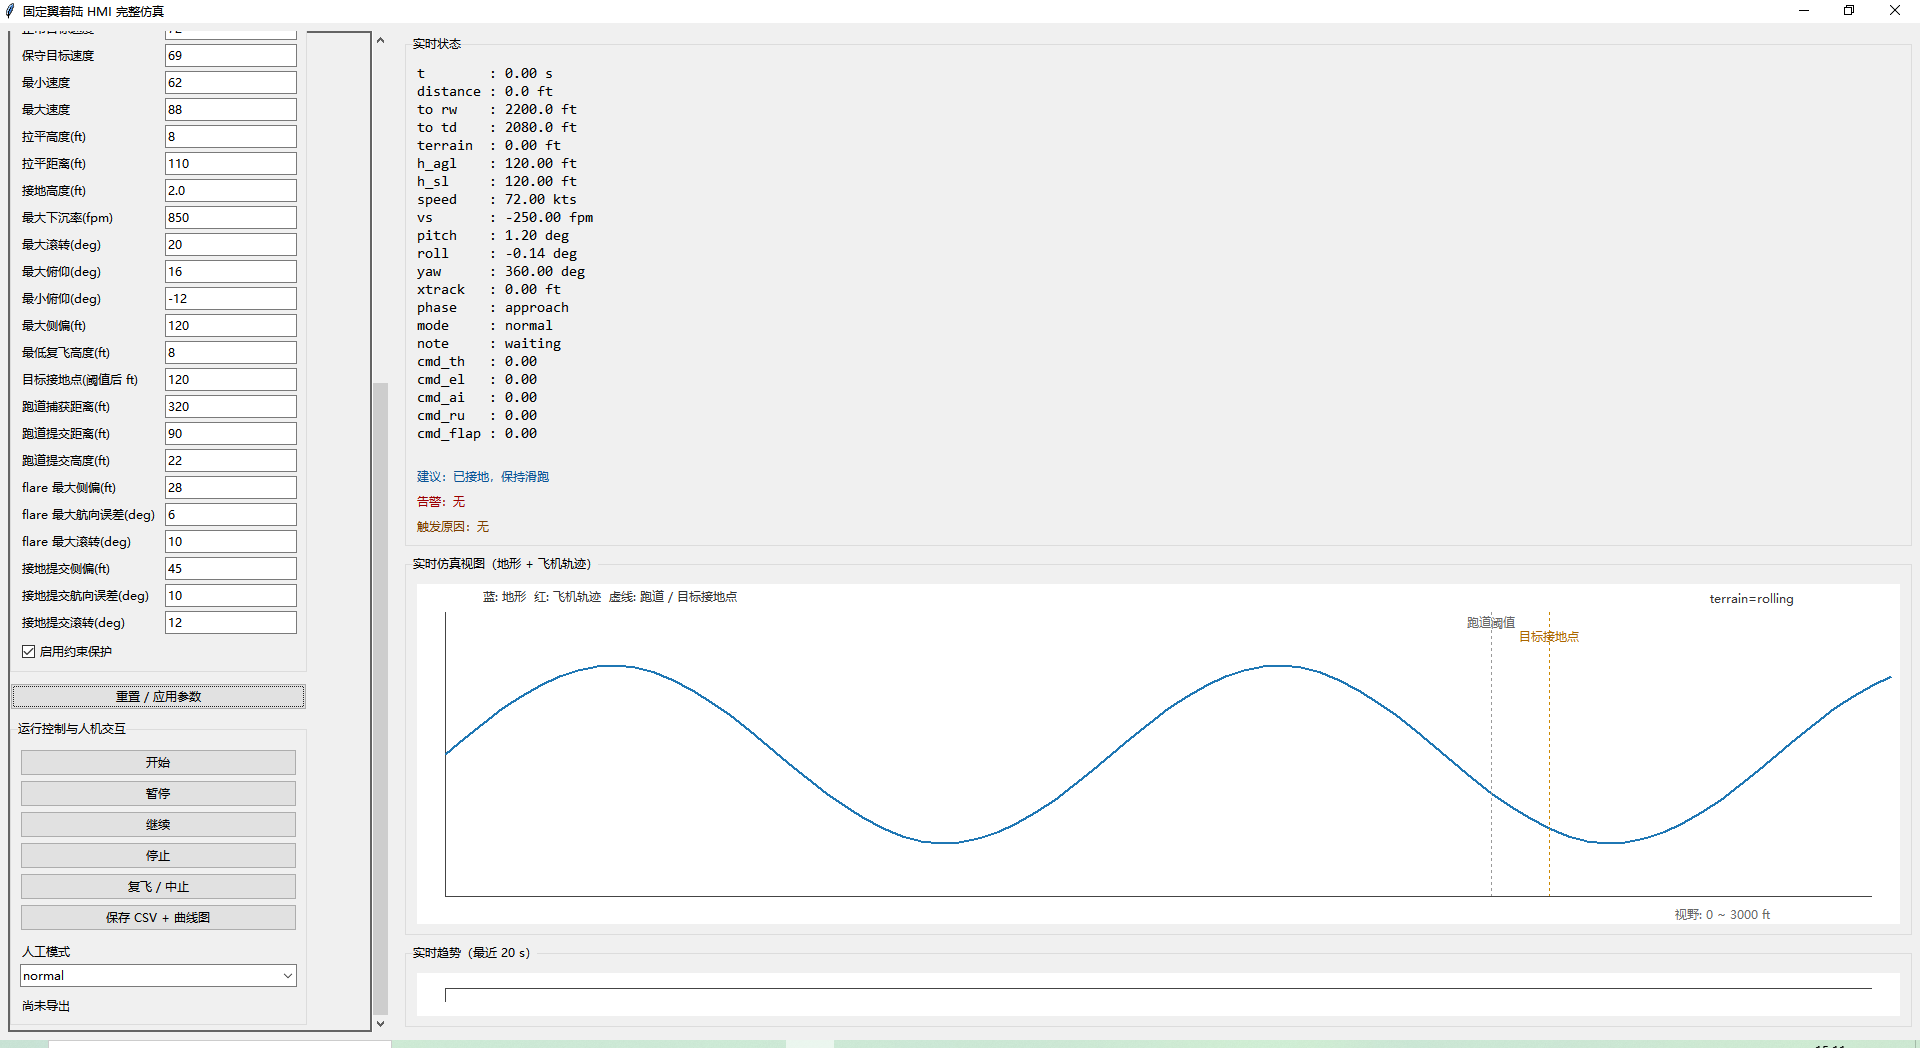
\includegraphics[width=4.19in,height=0.66\textheight,keepaspectratio]{images/image5.png}
\caption{固定翼着陆控制HMI仿真平台界面}
\label{fig:3-1}
\end{figure}

图~\ref{fig:3-1}为本文搭建的固定翼着陆控制仿真平台界面。界面主要包括参数输入区、运行控制区、实时状态显示区以及地形与轨迹显示区，可用于完成参数设置、过程监视和结果分析。

\section{数学模型与输出量定义}

基于上述等效模型，本文建立了纵向运动模型、侧向运动模型。纵向模型着重对飞行器在着陆进程里的速度、高度、下沉率还有俯仰角的变化予以描述，侧向模型主要针对滚转角、航向角、侧偏量的变化展开描述。结合仿真平台的相关参数，本文把下滑角设定为3.0$^\circ$，正常目标速度确定为72
kts，保守目标速度设定成69 kts，最小安全速度规定为62
kts，最大速度设置为88 kts，将拉平高度设定为8 ft，拉平距离定为110
ft，接地高度设为2 ft。这些参数足以满足本文着陆控制仿真分析的需求。

本文针对侧向控制参数设定了边界条件。把最大滚转角定为20$^\circ$，最大俯仰角确定为16$^\circ$，最小俯仰角设定成-12$^\circ$，最大侧偏量设为120
ft。当进入接地区域之后，系统采取更为严格的对准、姿态约束，以此提高着陆的安全性与稳定性。通过这样的做法，模型不但能够反映飞行器进近阶段的纠偏能力，还能够体现近地阶段对平稳接地的要求。

基于论文研究的具体内容，本文把输出量划分成了三类。其一为飞行状态量，其中涵盖了时间、距离、离地的高度、速度、下沉率、俯仰角、滚转角、航向角、侧偏量。其二是控制指令量，具体有油门、升降舵、副翼、方向舵、襟翼指令。其三是交互信息量，包括飞行阶段、提示信息、告警信息、触发原因等。梅荣于无人机起落架着陆缓冲性能优化及试验验证研究里提到，着陆分析需要同时关注飞行状态、接地品质，以此提高仿真结果的完整性。于是，本文在定义输出量的时候兼顾了飞行状态分析与交互提示分析这两方面的内容。

\begingroup\small
\begin{longtable}{@{}
  >{\raggedright\arraybackslash}p{(\columnwidth - 4\tabcolsep) * \real{0.3333}}
  >{\raggedright\arraybackslash}p{(\columnwidth - 4\tabcolsep) * \real{0.3334}}
  >{\raggedright\arraybackslash}p{(\columnwidth - 4\tabcolsep) * \real{0.3334}}@{}}
\caption{仿真平台主要参数设置}\label{tab:3-1}\\
\toprule\noalign{}
\begin{minipage}[b]{\linewidth}\raggedright
参数名称
\end{minipage} & \begin{minipage}[b]{\linewidth}\raggedright
数值
\end{minipage} & \begin{minipage}[b]{\linewidth}\raggedright
单位
\end{minipage} \\
\midrule\noalign{}
\endhead
\bottomrule\noalign{}
\endlastfoot
初始离地高度 & 120 & ft \\
初始速度 & 72 & kts \\
初始下降率 & -250 & fpm \\
下滑角 & 3.0 & $^\circ$ \\
正常目标速度 & 72 & kts \\
保守目标速度 & 69 & kts \\
最小安全速度 & 62 & kts \\
最大允许速度 & 88 & kts \\
拉平高度 & 8 & ft \\
拉平距离 & 110 & ft \\
接地高度 & 2 & ft \\
最大下沉率约束 & 850 & fpm \\
最大滚转角 & 20 & $^\circ$ \\
最大俯仰角 & 16 & $^\circ$ \\
最小俯仰角 & -12 & $^\circ$ \\
最大侧偏量 & 120 & ft \\
\end{longtable}
\endgroup

表~\ref{tab:3-1}为本文仿真平台采用的主要参数设置。这些参数用于统一各工况下的分析条件，为后续工况比较提供基础。

\section{仿真平台实现与参数化设置}

为了验证模型的有效性，本文依据已有的程序搭建了固定翼飞行器着陆控制仿真平台。这个平台拥有参数输入、控制计算、状态刷新、实时显示、数据导出还有结果绘图等功能，可以满足着陆控制系统仿真分析的需求。平台整体是由参数设置模块、控制器模块、环境与地形模块、状态显示模块、结果输出模块构成的，其中参数设置模块用来输入飞行初始条件和控制边界，控制器模块负责实时生成控制指令，环境模块承担建立不同地形条件的任务，结果输出模块用于保存CSV数据和仿真曲线图。

通过结合上传的仿真结果能够发现，不同地形条件下飞行器的着陆过程有着显著不同。在平坦地形时，AGL曲线整体下降比较平稳，速度、姿态的变化同样比较平顺，处于起伏地形和山脊地形时，离地高度变化更快，姿态修正更为频繁，谷地和阶跃地形会对近地区域的高度判断、拉平时机造成影响。这显示出复杂地形会加大着陆控制的难度，也进一步表明在人机交互强化条件下展开仿真分析是很有必要的。

\begin{figure}[H]
\centering
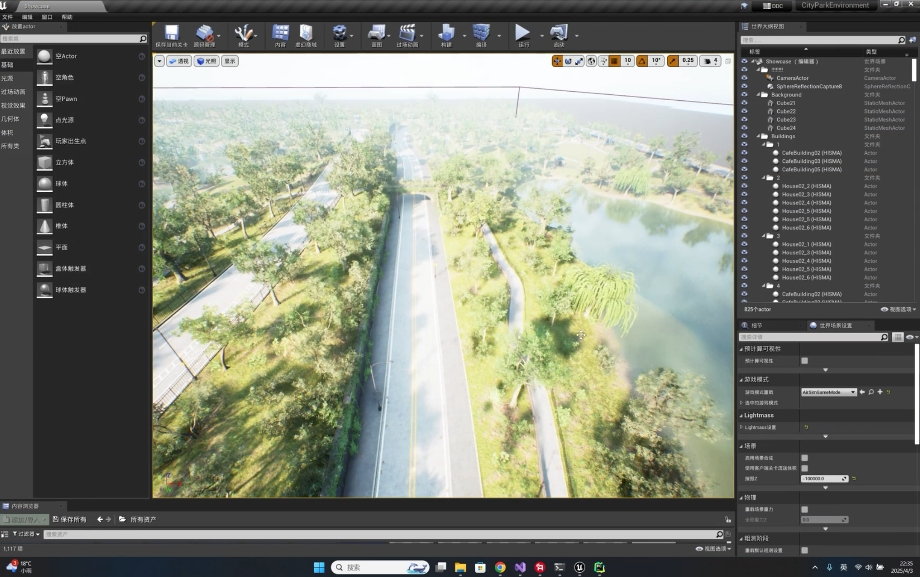
\includegraphics[width=0.92\linewidth,height=0.66\textheight,keepaspectratio]{images/image6.jpg}
\caption{仿真平台搭建}
\label{fig:3-2}
\end{figure}

\begin{figure}[H]
\centering
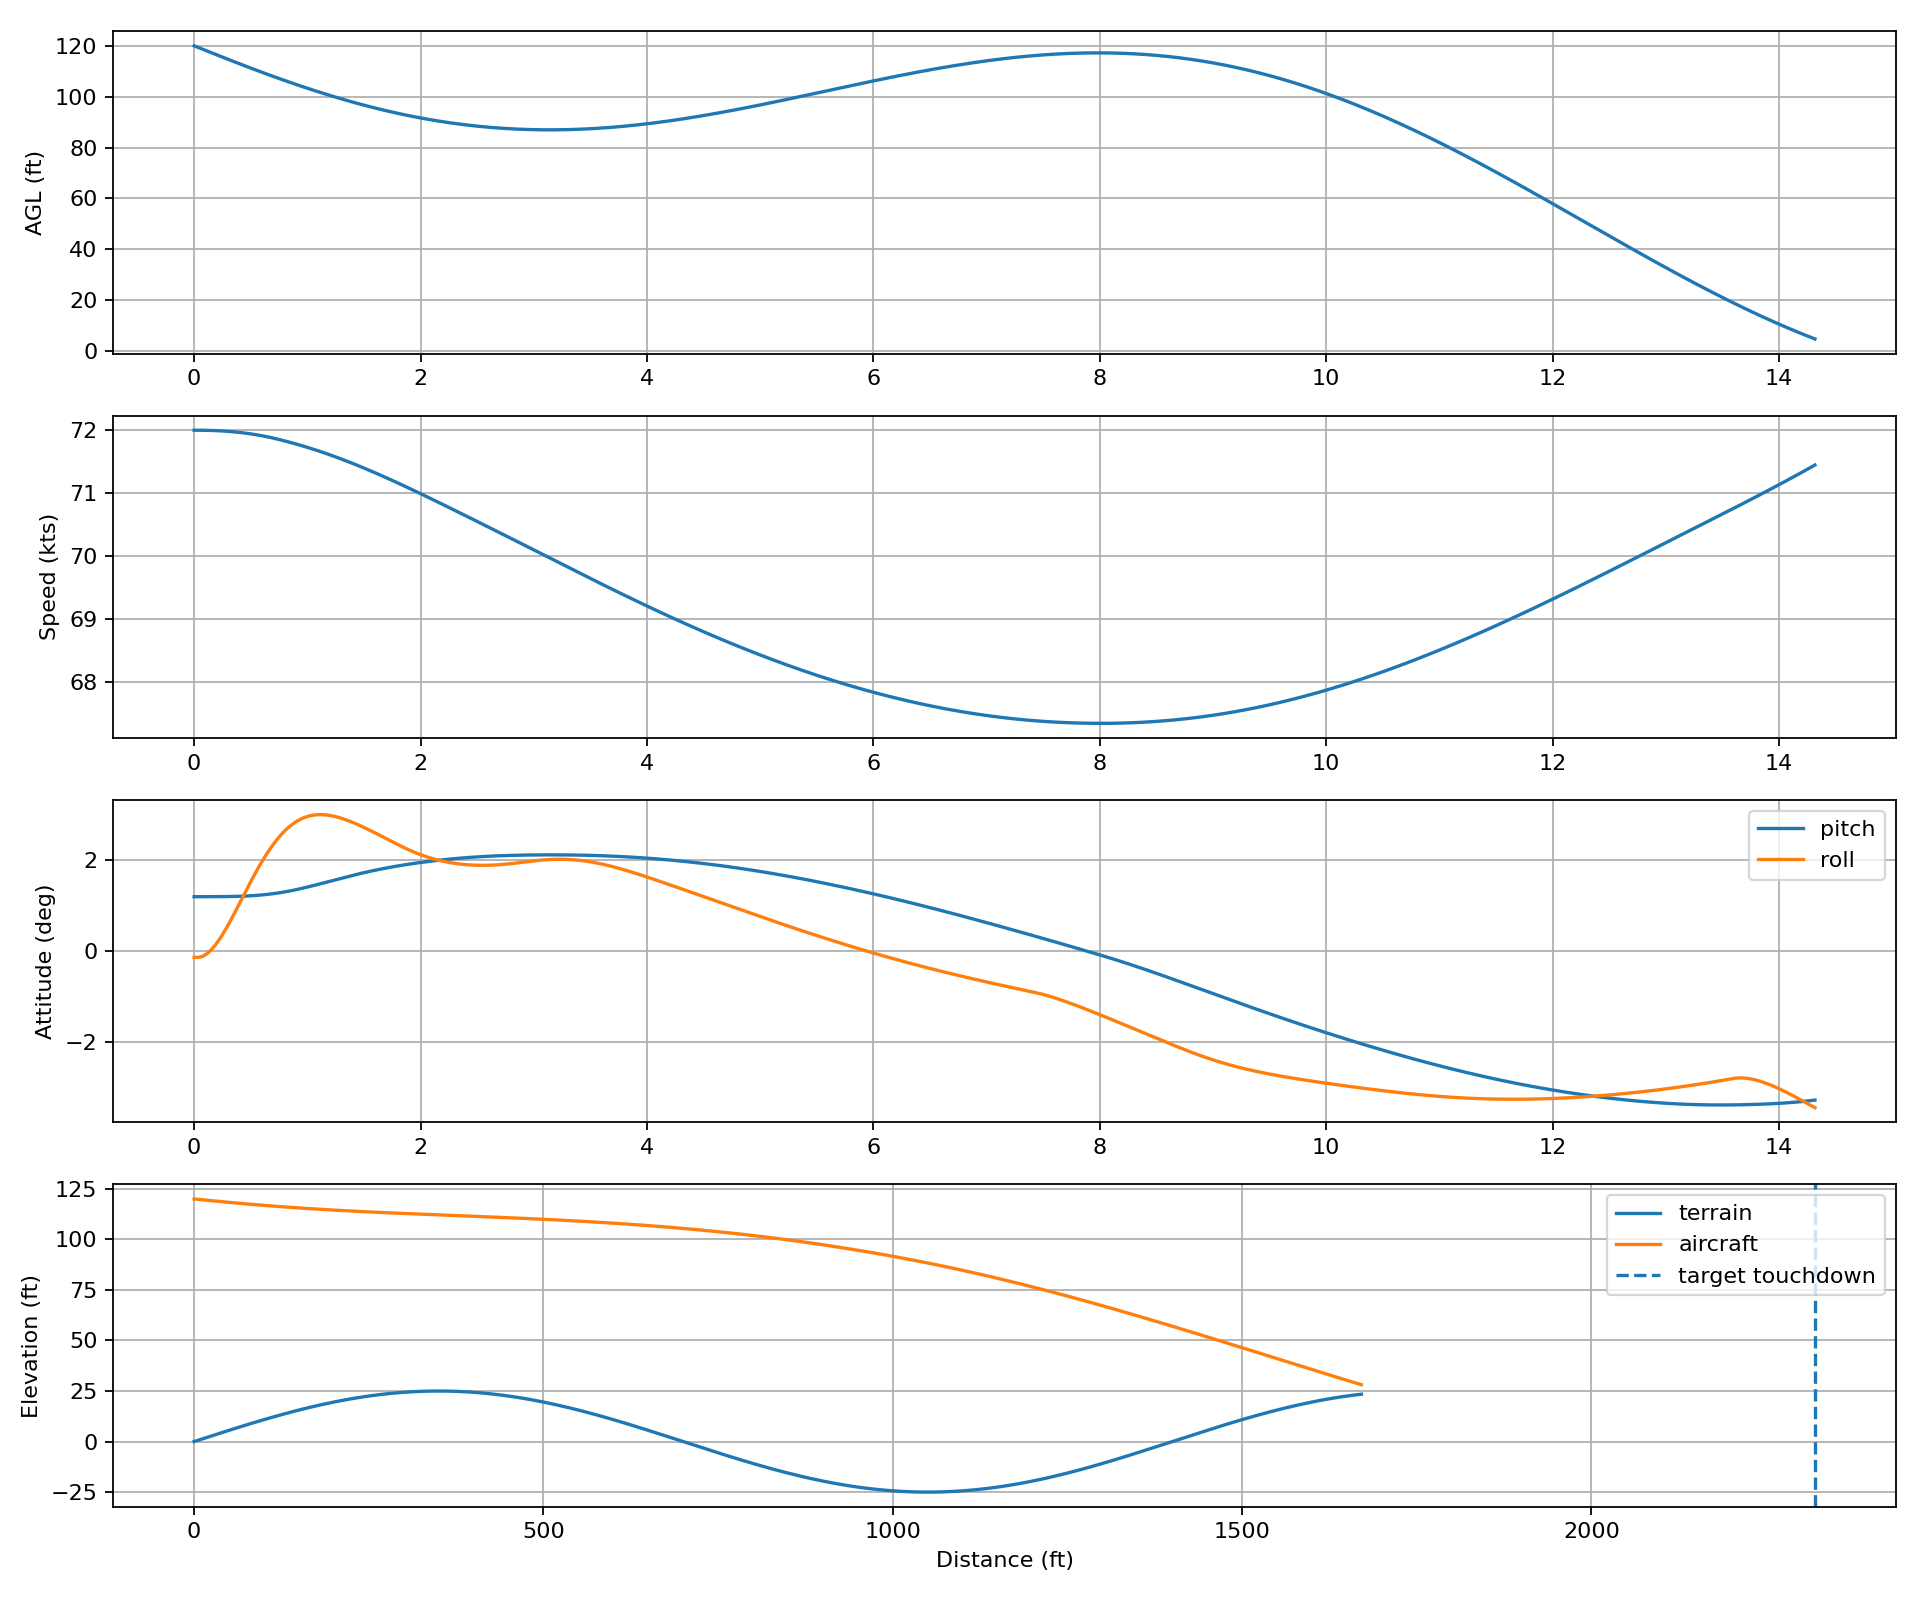
\includegraphics[width=4.00in,height=0.66\textheight,keepaspectratio]{images/image7.png}
\caption{平坦地形基准工况仿真结果}
\label{fig:3-3}
\end{figure}

图~\ref{fig:3-3}表明，在平坦地形工况下，飞行器着陆过程整体较为平稳，适合作为后续工况对比分析的基准工况。

\begin{figure}[H]
\centering
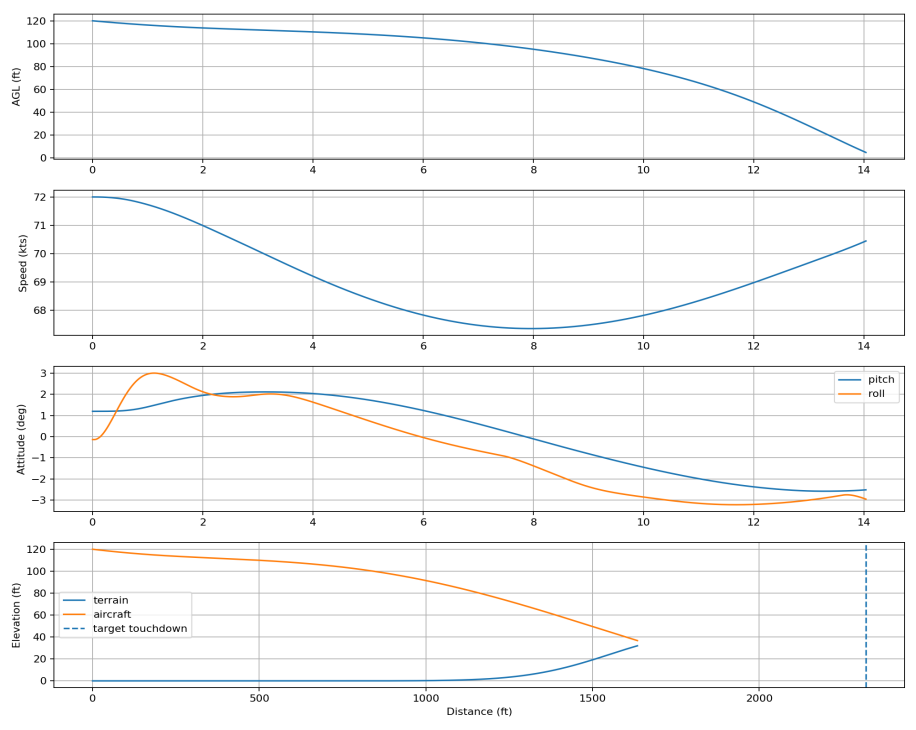
\includegraphics[width=4.16in,height=0.66\textheight,keepaspectratio]{images/image8.png}
\caption{起伏地形工况仿真结果}
\label{fig:3-4}
\end{figure}

图~\ref{fig:3-4}显示，起伏地形会使飞行器相对离地高度变化更加明显，从而增加着陆后段的控制难度。

\begin{figure}[H]
\centering
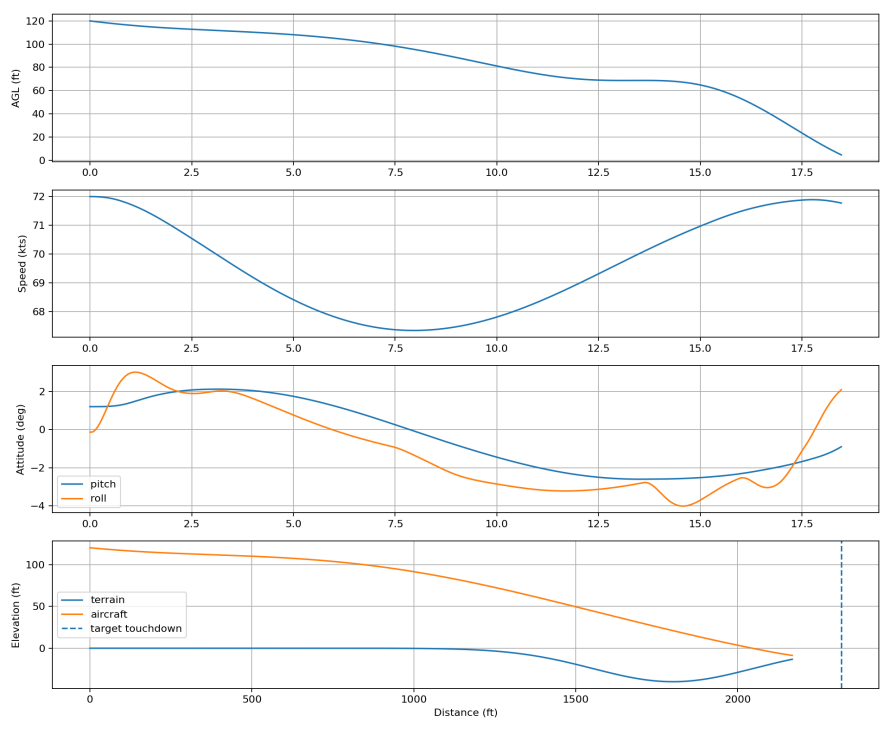
\includegraphics[width=4.05in,height=0.66\textheight,keepaspectratio]{images/image9.png}
\caption{山脊地形工况仿真结果}
\label{fig:3-5}
\end{figure}

图~\ref{fig:3-5}说明，山脊地形会使飞行器在接近着陆区域时面临地形快速抬升，对轨迹保持和姿态修正提出更高要求。

\begin{figure}[H]
\centering
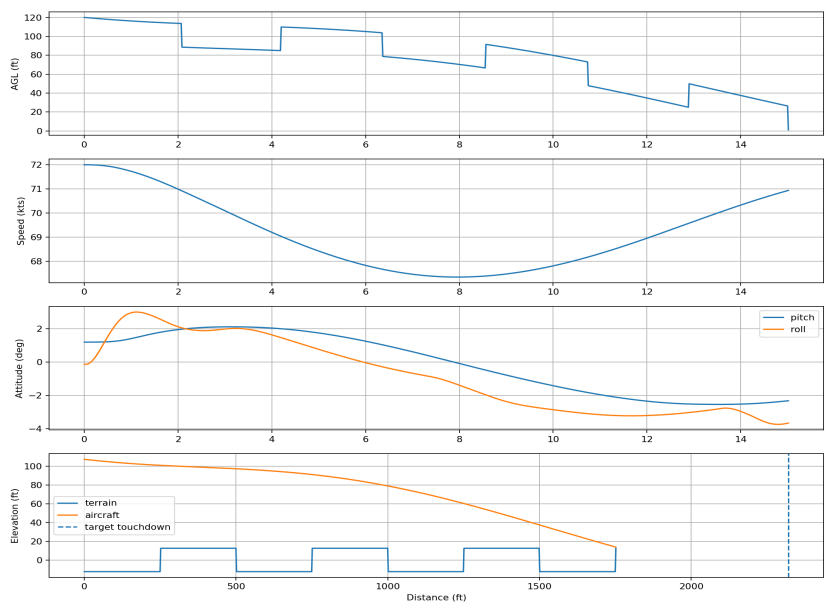
\includegraphics[width=3.79in,height=0.66\textheight,keepaspectratio]{images/image10.png}
\caption{谷地地形工况仿真结果}
\label{fig:3-6}
\end{figure}

图~\ref{fig:3-6}表明，谷地地形会改变飞行器末段离地高度变化规律，使操纵者对拉平时机的判断更加复杂。

\begin{figure}[H]
\centering
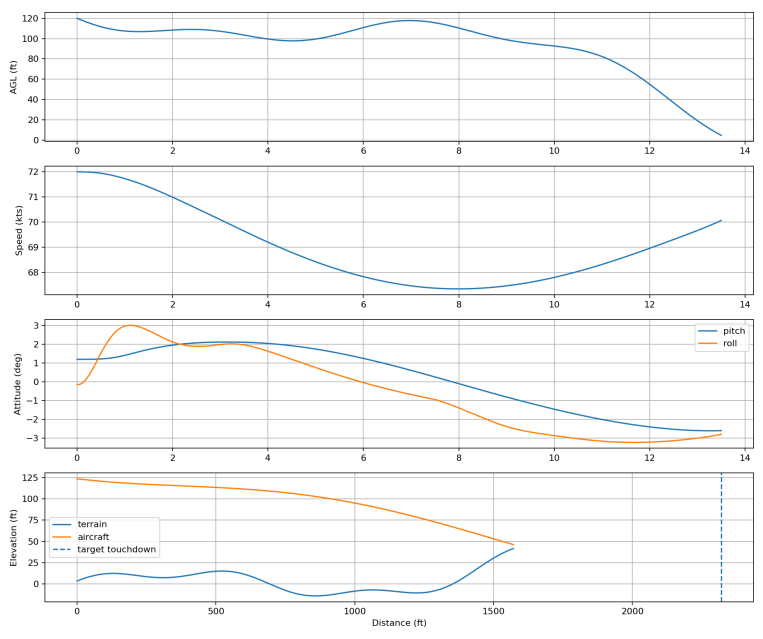
\includegraphics[width=3.47in,height=0.66\textheight,keepaspectratio]{images/image11.png}
\caption{阶跃地形工况仿真结果}
\label{fig:3-7}
\end{figure}

图~\ref{fig:3-7}显示，阶跃地形会使飞行器相对离地高度出现突变特征，从而对着陆阶段的稳定控制产生影响。

为了便于比较不同地形工况下的仿真结果，本文对关键指标进行了整理，如表~\ref{tab:3-2}所示。

\begingroup\small
\begin{longtable}{@{}
  >{\raggedright\arraybackslash}p{(\columnwidth - 10\tabcolsep) * \real{0.1666}}
  >{\raggedright\arraybackslash}p{(\columnwidth - 10\tabcolsep) * \real{0.1666}}
  >{\raggedright\arraybackslash}p{(\columnwidth - 10\tabcolsep) * \real{0.1666}}
  >{\raggedright\arraybackslash}p{(\columnwidth - 10\tabcolsep) * \real{0.1666}}
  >{\raggedright\arraybackslash}p{(\columnwidth - 10\tabcolsep) * \real{0.1667}}
  >{\raggedright\arraybackslash}p{(\columnwidth - 10\tabcolsep) * \real{0.1667}}@{}}
\caption{不同地形工况关键仿真结果对比}\label{tab:3-2}\\
\toprule\noalign{}
\begin{minipage}[b]{\linewidth}\raggedright
工况类型
\end{minipage} & \begin{minipage}[b]{\linewidth}\raggedright
仿真时长/s
\end{minipage} & \begin{minipage}[b]{\linewidth}\raggedright
最终AGL/ft
\end{minipage} & \begin{minipage}[b]{\linewidth}\raggedright
末段速度/kts
\end{minipage} & \begin{minipage}[b]{\linewidth}\raggedright
末段俯仰角/($^\circ$)
\end{minipage} & \begin{minipage}[b]{\linewidth}\raggedright
末段滚转角/($^\circ$)
\end{minipage} \\
\midrule\noalign{}
\endhead
\bottomrule\noalign{}
\endlastfoot
平坦地形 & 17.15 & 4.60 & 71.80 & -1.28 & -2.28 \\
起伏地形 & 14.32 & 4.70 & 71.45 & -3.29 & -3.45 \\
山脊地形 & 14.03 & 4.74 & 70.44 & -2.52 & -2.96 \\
谷地地形 & 18.47 & 4.60 & 71.78 & -0.90 & 2.09 \\
阶跃地形 & 15.02 & 1.20 & 70.94 & -2.33 & -3.67 \\
\end{longtable}
\endgroup

由表~\ref{tab:3-2}可以看出，不同地形条件下系统输出结果存在明显差异。起伏地形工况的最大下沉率绝对值最大，说明其对着陆纵向控制影响更突出；谷地地形工况的最大滚转角最大，说明其对姿态控制和横向稳定性影响更明显；阶跃地形工况最终AGL最低，反映出地形突变对末段离地高度判断的干扰最强。因此，在后续工况设计与评价分析中，有必要把复杂地形作为重点考察对象，并结合人机交互强化策略进一步分析其对着陆品质改善的作用。

本文仿真平台在参数配置、控制逻辑方面保留了工程可扩展性。比如说能够进一步借助调整缓冲边界参数、接地阈值、风险触发条件，去模拟不同起落架构型、不同着陆策略之下的响应差异。赵知辛等人在仿竹设计无人机起落架结构中的应用研究显示，起落架系统设计不但关乎结构轻量化，而且对接地吸能、冲击适应能力也有影响。受此启发，本文虽说重点研究的是着陆控制系统与人机交互强化，不过在仿真平台设置里依旧保留了对接地边界、缓冲安全性、复杂地形适应性的关注，进而为后续系统优化分析提供更为完整的基础。

%!TEX root = ../hutbthesis_main.tex

\chapter{模型校核、性能评价方法与工况设计}

\section{基准工况自检与模型校核}

进行多工况仿真分析之前，要先针对着陆控制动力学模型进行基准工况自检、模型校核工作，目的是确保后续结果具备可比性与可信性。本文把平坦地形、正常模式、无初始侧偏、无额外航向误差选作基准工况。其参数设定如下：初始离地高度为120
ft，初始速度是72 kts，初始下降率为-250 fpm，跑道距离为2200
ft，下滑角为3.0$^\circ$，目标接地点设定在跑道阈值后120
ft处，同时开启约束保护逻辑。

依据仿真结果可知，在基准工况时飞行器能够沿着预定的下滑轨迹实现稳定下降，其离地高度随着时间持续减小，速度维持在安全范围之内，俯仰角、滚转角的变化较小，这表明该模型在纵向控制还有侧向控制方面整体比较协调。当进入着陆末段之后，系统能够及时从进近阶段转换至拉平阶段，并且在接地区域优先执行稳定接地逻辑，没有出现明显的轨迹突变或者状态发散情况。已有结果显示，在该工况下仿真时长大约是17.15
s，末段离地高度约为4.60 ft，末段速度约为71.80
kts，末段俯仰角约为-1.28$^\circ$，末段滚转角约为-2.28$^\circ$。这些数据表明模型在标准条件下运行稳定，能够满足后续复杂工况分析的需求。

模型校核主要有三个方向：其一为轨迹合理性，也就是查看飞行器能否顺着预定下滑路径持续靠近跑道，其二是状态边界合理性，即检验速度、下沉率、姿态角、侧偏量是否处于合理区间，其三是阶段切换合理性，即核查系统是否能够在适宜的高度和距离进入flare阶段，并在近地区域维持以稳定接地为主的控制策略。精确着陆研究通常觉得，着陆控制模型是否可靠，既体现在轨迹能否闭合，也体现在关键状态量是否处在可接受窗口内。所以，本文经由基准工况的自检来确认模型拥有后续多工况比较的基本条件。

\begin{figure}[H]
\centering
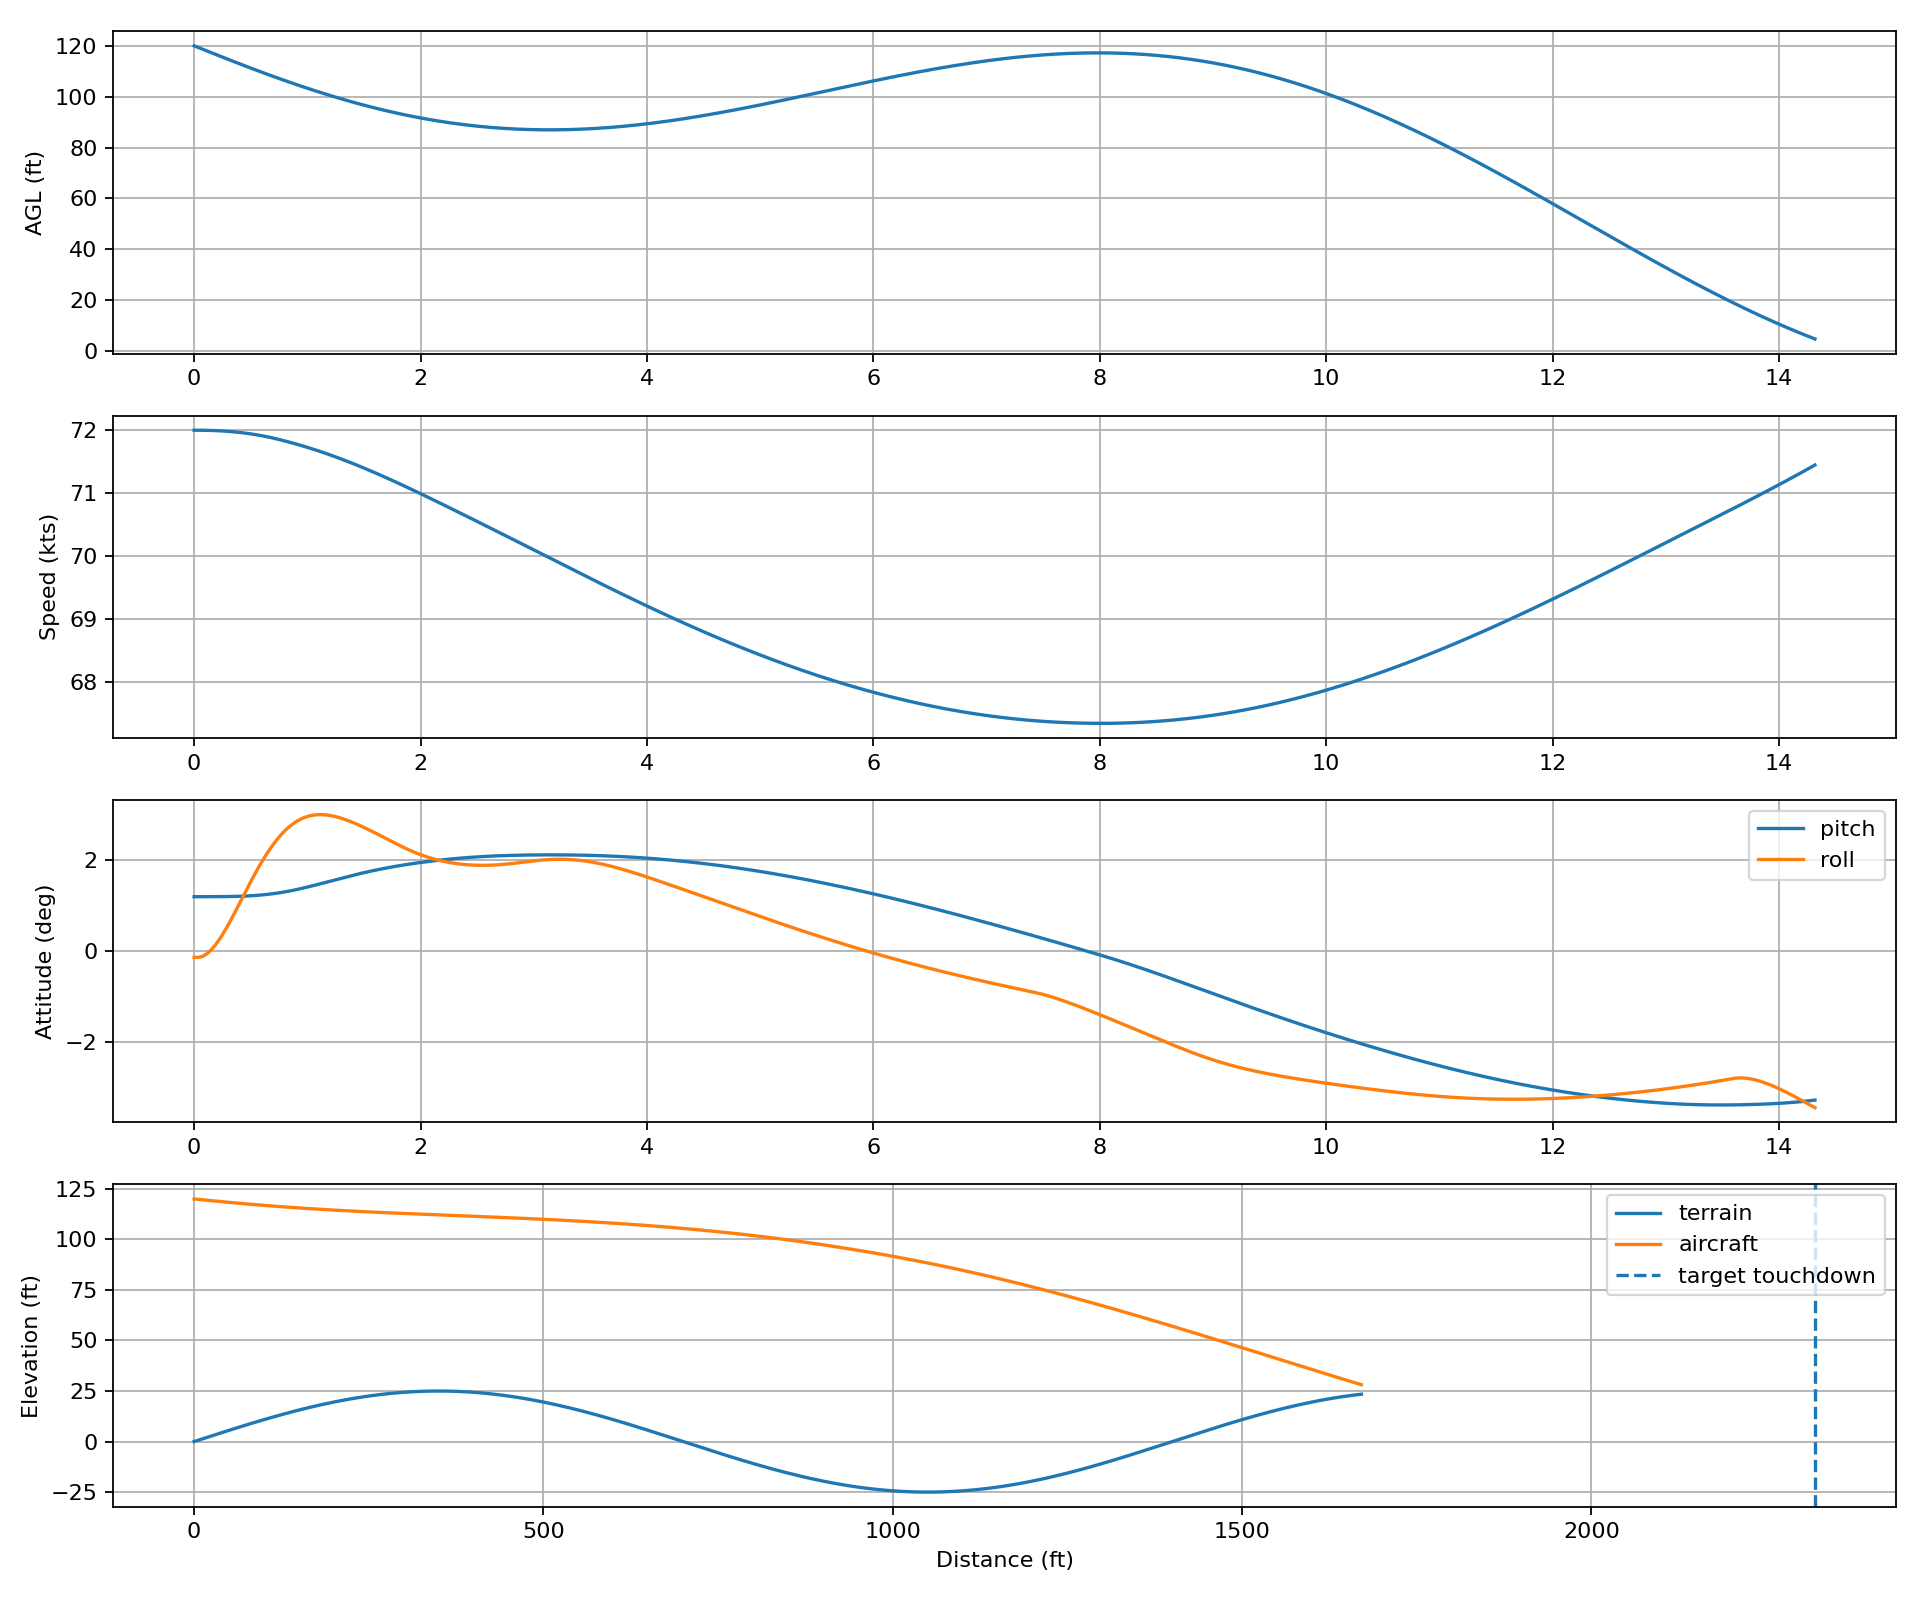
\includegraphics[width=3.47in,height=0.66\textheight,keepaspectratio]{images/image7.png}
\caption{基准工况模型校核结果图}
\label{fig:4-1}
\end{figure}

图~\ref{fig:4-1}反映了基准工况下飞行器AGL、速度、姿态角及轨迹变化情况。由图可见，飞行器在标准条件下状态收敛较好，说明模型校核结果满足后续分析要求。

\section{评价指标与判据建立}

为系统评价不同工况下固定翼飞行器着陆控制系统的性能，本文建立了评价指标模式，该模式包括安全性、稳定性、精度、交互有效性这四个方面。安全性指标包括飞行速度、最大下沉率、俯仰角与滚转角。稳定性指标涵盖离地高度变化是否连续、轨迹是否平滑、阶段切换是否合理。精度指标有侧偏量、航向误差、目标接地点附近位置的控制情况。交互有效性指标包括提示信息、告警触发、约束保护是否及时有效。

依据仿真平台的各项参数，本文确定了以下基本判据。在飞行速度处于62至88节这个范围，并且最大下沉率不超过850英尺每分钟，同时滚转角的绝对值不超过20度、俯仰角保持在负12度至16度之间的时候，判定系统符合基本飞行安全要求。当飞行器进入flare阶段之后，如果侧偏量不超过28英尺、航向误差不超过6度、滚转角不超过10度，那就判定拉平阶段横向对准状态良好。当进入接地提交阶段后，要是侧偏量不超过45英尺、航向误差不超过10度、滚转角不超过12度，便认为系统满足稳定接地要求。要是单项指标出现局部超限的情形，可判定为性能有所下降，要是多项关键指标同时超限，或者系统触发了复飞/中止逻辑，那么可判定为不利工况。

建立评价模式时，本文对着陆任务场景特点予以充分考虑。固定翼飞行器着陆属于典型的末段精确控制任务，仅靠单一指标不能全面展现系统性能，因此需把速度、姿态、侧偏及阶段切换等指标结合起来做综合评判。郑金豪在无人机精确着陆控制技术研究里指出，精确着陆的关键在于多状态量联合约束与分阶段控制协调。所以，本文建立的评价判据既关注单个状态量有无超出限定，也留意其在不同阶段的综合表现状况。

\begingroup\small
\begin{longtable}{@{}
  >{\raggedright\arraybackslash}p{(\columnwidth - 4\tabcolsep) * \real{0.3333}}
  >{\raggedright\arraybackslash}p{(\columnwidth - 4\tabcolsep) * \real{0.3334}}
  >{\raggedright\arraybackslash}p{(\columnwidth - 4\tabcolsep) * \real{0.3334}}@{}}
\caption{着陆性能评价指标与判据}\label{tab:4-1}\\
\toprule\noalign{}
\begin{minipage}[b]{\linewidth}\raggedright
指标类别
\end{minipage} & \begin{minipage}[b]{\linewidth}\raggedright
指标名称
\end{minipage} & \begin{minipage}[b]{\linewidth}\raggedright
判据
\end{minipage} \\
\midrule\noalign{}
\endhead
\bottomrule\noalign{}
\endlastfoot
安全性 & 飞行速度 & 62～88 kts \\
安全性 & 最大下沉率 & 不大于850 fpm \\
安全性 & 滚转角 & \textbar roll\textbar$\leq$20$^\circ$ \\
安全性 & 俯仰角 & -12$^\circ$～16$^\circ$ \\
精度 & flare阶段侧偏量 & $\leq$28 ft \\
精度 & flare阶段航向误差 & $\leq$6$^\circ$ \\
精度 & 接地提交侧偏量 & $\leq$45 ft \\
精度 & 接地提交航向误差 & $\leq$10$^\circ$ \\
稳定性 & 阶段切换 & 平滑、无明显突变 \\
交互有效性 & 告警与约束触发 & 及时、准确 \\
\end{longtable}
\endgroup

表~\ref{tab:4-1}给出了本文采用的主要评价指标与判据。后续各工况仿真结果均以该指标体系为基础进行横向比较和优劣识别。

\section{工况矩阵设计}

为剖析不同条件下模型的响应规律，本文依据已有的平台参数、仿真结果，设计了包括``地形条件
+ 控制模式 +
边界扰动''的工况矩阵。在地形条件这一方面，挑选了平坦地形、起伏地形、山脊地形、谷地地形、阶跃地形这五种具有代表性的环境，以此来呈现不同地面高程变化给着陆控制带来的影响，在控制模式上，设定了正常模式和保守模式这两种模式，用来探究不同目标速度策略下系统的性能差异，针对边界扰动，可以增加初始侧偏、航向误差或者较大下沉率等因素，从而建立更为复杂的工况场景。

在本文的基础工况里，主要是对五类地形展开对比，其他参数维持不变，以此来突出地形因素所产生的影响。为了验证控制系统对于不同进近地形扰动的适应能力，在本节当中设计了六类地形剖面，分别是平坦、起伏、山脊、谷地、阶跃、混合地形剖面，并且让初始高度保持在120英尺、速度维持在72节、跑道距离设定为2200英尺不变。将平坦地形用作基准参考，起伏地形用来分析连续高程变化对着地高度、姿态调节所造成的影响，山脊地形用于分析近地高程快速抬升时系统的应对状况，谷地地形用来分析先缓后急的相对离地高度变化情况，阶跃地形用于模拟局部高程突变对末段判断形成的干扰。借助这样的方式，便能够比较展现出不同场景下着陆控制系统的适应性能。

\begin{figure}[H]
\centering
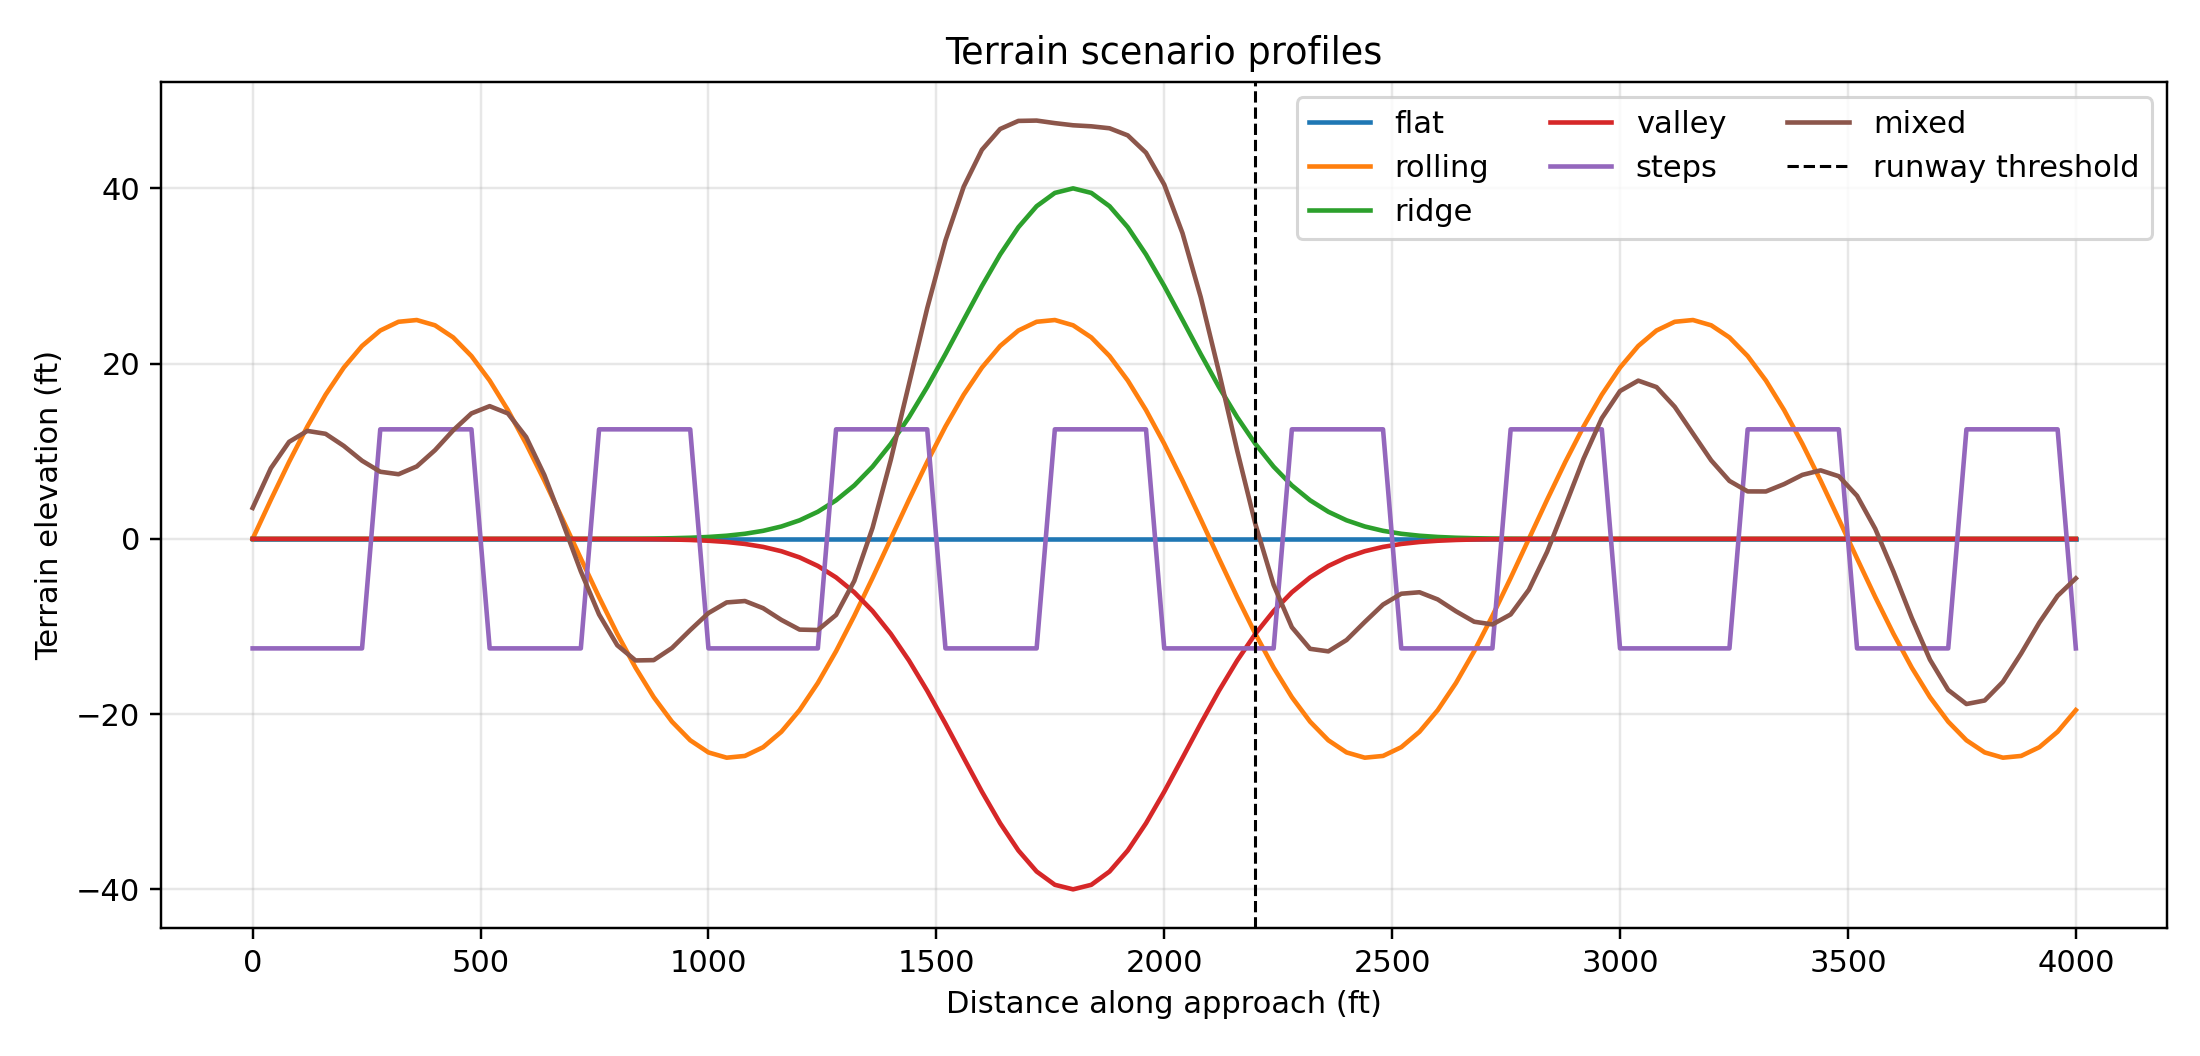
\includegraphics[width=0.92\linewidth,height=0.66\textheight,keepaspectratio]{images/image12.png}
\caption{不同地形工况的跑道进近剖面对比}
\label{fig:4-2}
\end{figure}

同时，为了体现工况设计的合理性，本文在矩阵设置中保留了由``标准条件''到``复杂条件''的渐进关系。先利用基础地形工况完成模型特性识别，再通过增加初始侧偏和下沉率偏差等方式扩展复杂工况。周乐等在仿生四足六旋翼无人机自适应着陆性能分析中指出，不同着陆场景对系统适应能力的要求具有明显差异，应通过多场景测试来识别系统的优势与薄弱环节。虽然本文对象为固定翼飞行器，但其工况设计思路同样适用，即通过典型场景组合提高评价的完整性。

\begingroup\small
\begin{longtable}{@{}
  >{\raggedright\arraybackslash}p{(\columnwidth - 10\tabcolsep) * \real{0.1666}}
  >{\raggedright\arraybackslash}p{(\columnwidth - 10\tabcolsep) * \real{0.1666}}
  >{\raggedright\arraybackslash}p{(\columnwidth - 10\tabcolsep) * \real{0.1666}}
  >{\raggedright\arraybackslash}p{(\columnwidth - 10\tabcolsep) * \real{0.1666}}
  >{\raggedright\arraybackslash}p{(\columnwidth - 10\tabcolsep) * \real{0.1667}}
  >{\raggedright\arraybackslash}p{(\columnwidth - 10\tabcolsep) * \real{0.1667}}@{}}
\caption{仿真工况矩阵设计}\label{tab:4-2}\\
\toprule\noalign{}
\begin{minipage}[b]{\linewidth}\raggedright
工况编号
\end{minipage} & \begin{minipage}[b]{\linewidth}\raggedright
地形类型
\end{minipage} & \begin{minipage}[b]{\linewidth}\raggedright
控制模式
\end{minipage} & \begin{minipage}[b]{\linewidth}\raggedright
初始侧偏
\end{minipage} & \begin{minipage}[b]{\linewidth}\raggedright
初始下降率
\end{minipage} & \begin{minipage}[b]{\linewidth}\raggedright
分析目标
\end{minipage} \\
\midrule\noalign{}
\endhead
\bottomrule\noalign{}
\endlastfoot
C1 & 平坦地形 & normal & 0 ft & -250 fpm & 基准工况校核 \\
C2 & 起伏地形 & normal & 0 ft & -250 fpm & 连续高程变化影响 \\
C3 & 山脊地形 & normal & 0 ft & -250 fpm & 近地抬升影响 \\
C4 & 谷地地形 & normal & 0 ft & -250 fpm & 谷地环境影响 \\
C5 & 阶跃地形 & normal & 0 ft & -250 fpm & 地形突变影响 \\
C6 & 平坦地形 & conservative & 0 ft & -250 fpm & 保守速度策略效果 \\
C7 & 起伏地形 & normal & 20 ft & -250 fpm & 横向偏差影响 \\
C8 & 山脊地形 & normal & 0 ft & -400 fpm & 较大下沉率影响 \\
\end{longtable}
\endgroup

\section{仿真计算与数据整理}

在工况矩阵确定完毕之后，本文运用统一的参数口径来进行仿真计算工作，并且借助CSV导出、曲线图绘制的方式对结果加以整理。仿真输出所涵盖的内容主要有时间、飞行距离、跑道相对距离、目标接地点距离、离地高度、海拔高度、速度、下沉率、俯仰角、滚转角、航向角、侧偏量、控制指令、飞行阶段、提示与告警信息等。对这些数据予以整理之后，能够进一步提取出各工况下的末段速度、末段姿态、末段离地高度、阶段切换特征。

根据已有的基础工况成果，五类地形的主要数据情况是这样的。平坦地形工况下，仿真时长为十七点一五秒，末端的AGL大约是四点六零英尺，末端速度约为七十一点八零节。起伏地形工况的仿真时长为十四点三二秒，末端AGL约为四点七零英尺，末端速度约为七十一点四五节。山脊地形工况的仿真时长是十四点零三秒，末端AGL约为四点七四英尺，末端速度约为七十点四四节。谷地地形工况的仿真时长为十八点四七秒，末端AGL约是四点六零英尺，末端速度约为七十一点七八节。阶跃地形工况的仿真时长是十五点零二秒，末端AGL约为一点二零英尺，末端速度约为七十点九四节。从这些数据可以发现，不同地形状况下系统的输出有差别，其中阶跃地形对近地高度的判断影响较大，起伏地形和山脊地形对姿态修正、末端控制的影响比较明显。

\begingroup\small
\begin{longtable}{@{}
  >{\raggedright\arraybackslash}p{(\columnwidth - 10\tabcolsep) * \real{0.1666}}
  >{\raggedright\arraybackslash}p{(\columnwidth - 10\tabcolsep) * \real{0.1666}}
  >{\raggedright\arraybackslash}p{(\columnwidth - 10\tabcolsep) * \real{0.1666}}
  >{\raggedright\arraybackslash}p{(\columnwidth - 10\tabcolsep) * \real{0.1666}}
  >{\raggedright\arraybackslash}p{(\columnwidth - 10\tabcolsep) * \real{0.1667}}
  >{\raggedright\arraybackslash}p{(\columnwidth - 10\tabcolsep) * \real{0.1667}}@{}}
\caption{不同地形基础工况关键结果整理}\label{tab:4-3}\\
\toprule\noalign{}
\begin{minipage}[b]{\linewidth}\raggedright
地形工况
\end{minipage} & \begin{minipage}[b]{\linewidth}\raggedright
仿真时长/s
\end{minipage} & \begin{minipage}[b]{\linewidth}\raggedright
末段AGL/ft
\end{minipage} & \begin{minipage}[b]{\linewidth}\raggedright
末段速度/kts
\end{minipage} & \begin{minipage}[b]{\linewidth}\raggedright
末段俯仰角/($^\circ$)
\end{minipage} & \begin{minipage}[b]{\linewidth}\raggedright
末段滚转角/($^\circ$)
\end{minipage} \\
\midrule\noalign{}
\endhead
\bottomrule\noalign{}
\endlastfoot
平坦地形 & 17.15 & 4.60 & 71.80 & -1.28 & -2.28 \\
起伏地形 & 14.32 & 4.70 & 71.45 & -3.29 & -3.45 \\
山脊地形 & 14.03 & 4.74 & 70.44 & -2.52 & -2.96 \\
谷地地形 & 18.47 & 4.60 & 71.78 & -0.90 & 2.09 \\
阶跃地形 & 15.02 & 1.20 & 70.94 & -2.33 & -3.67 \\
\end{longtable}
\endgroup

由表~\ref{tab:4-3}可以看出，不同地形条件下系统输出存在明显差异。其中，起伏地形和山脊地形使飞行器姿态修正幅度更大，谷地地形使仿真持续时间相对较长，而阶跃地形对末段离地高度影响最突出。这些结果表明，本文所建立的模型和仿真平台能够较好地区分不同工况下的着陆响应差异，并为后续第5章``不利工况识别与机理解释''提供数据基础。

%!TEX root = ../hutbthesis_main.tex

\chapter{多工况仿真结果分析与不利工况识别}

\section{工况变化规律分析}

在前文模型校核、工况矩阵设计基础之上，本文就平坦地形、起伏地形、山脊地形、谷地地形和阶跃地形这五种基础工况展开对比分析。不同工况时飞行器着陆末段的离地高度、速度、姿态角、横向稳定性有差异，证明地形条件对固定翼飞行器着陆控制性能有直接影响。

从离地高度的变化规律方面来看，在平坦地形的工况之下，飞行器的AGL曲线变化是最为平缓的，在整个着陆过程当中，它是沿着预定的下滑轨迹持续下降的，其末段的控制过程比较稳定。在起伏地形的工况里，因为地面高程一直在变化，飞行器相对离地高度呈现出更为明显的非线性变化，使得系统在末段需要进行更为频繁的高度修正。在山脊地形的工况中，飞行器接近跑道区域之前，地面高程快速抬升，致使相对离地高度在短时间内明显减小，这对拉平时机提出了更高的要求。谷地地形的工况表现为前段高度裕度比较大而后段相对离地高度变化加快的特点，这种变化会增加后段控制节奏的复杂性。在阶跃地形的工况中，地面高程存在突变，让飞行器AGL变化出现明显的压缩特征，这对末段接地判断的影响是最大的。

图~\ref{fig:5-1}直观地对比了不同地形工况下离地高度与空速的响应曲线。可以看出，阶跃地形下近地高度余量最低，体现了突变地形对末端着陆安全裕度的影响。

\begin{figure}[H]
\centering
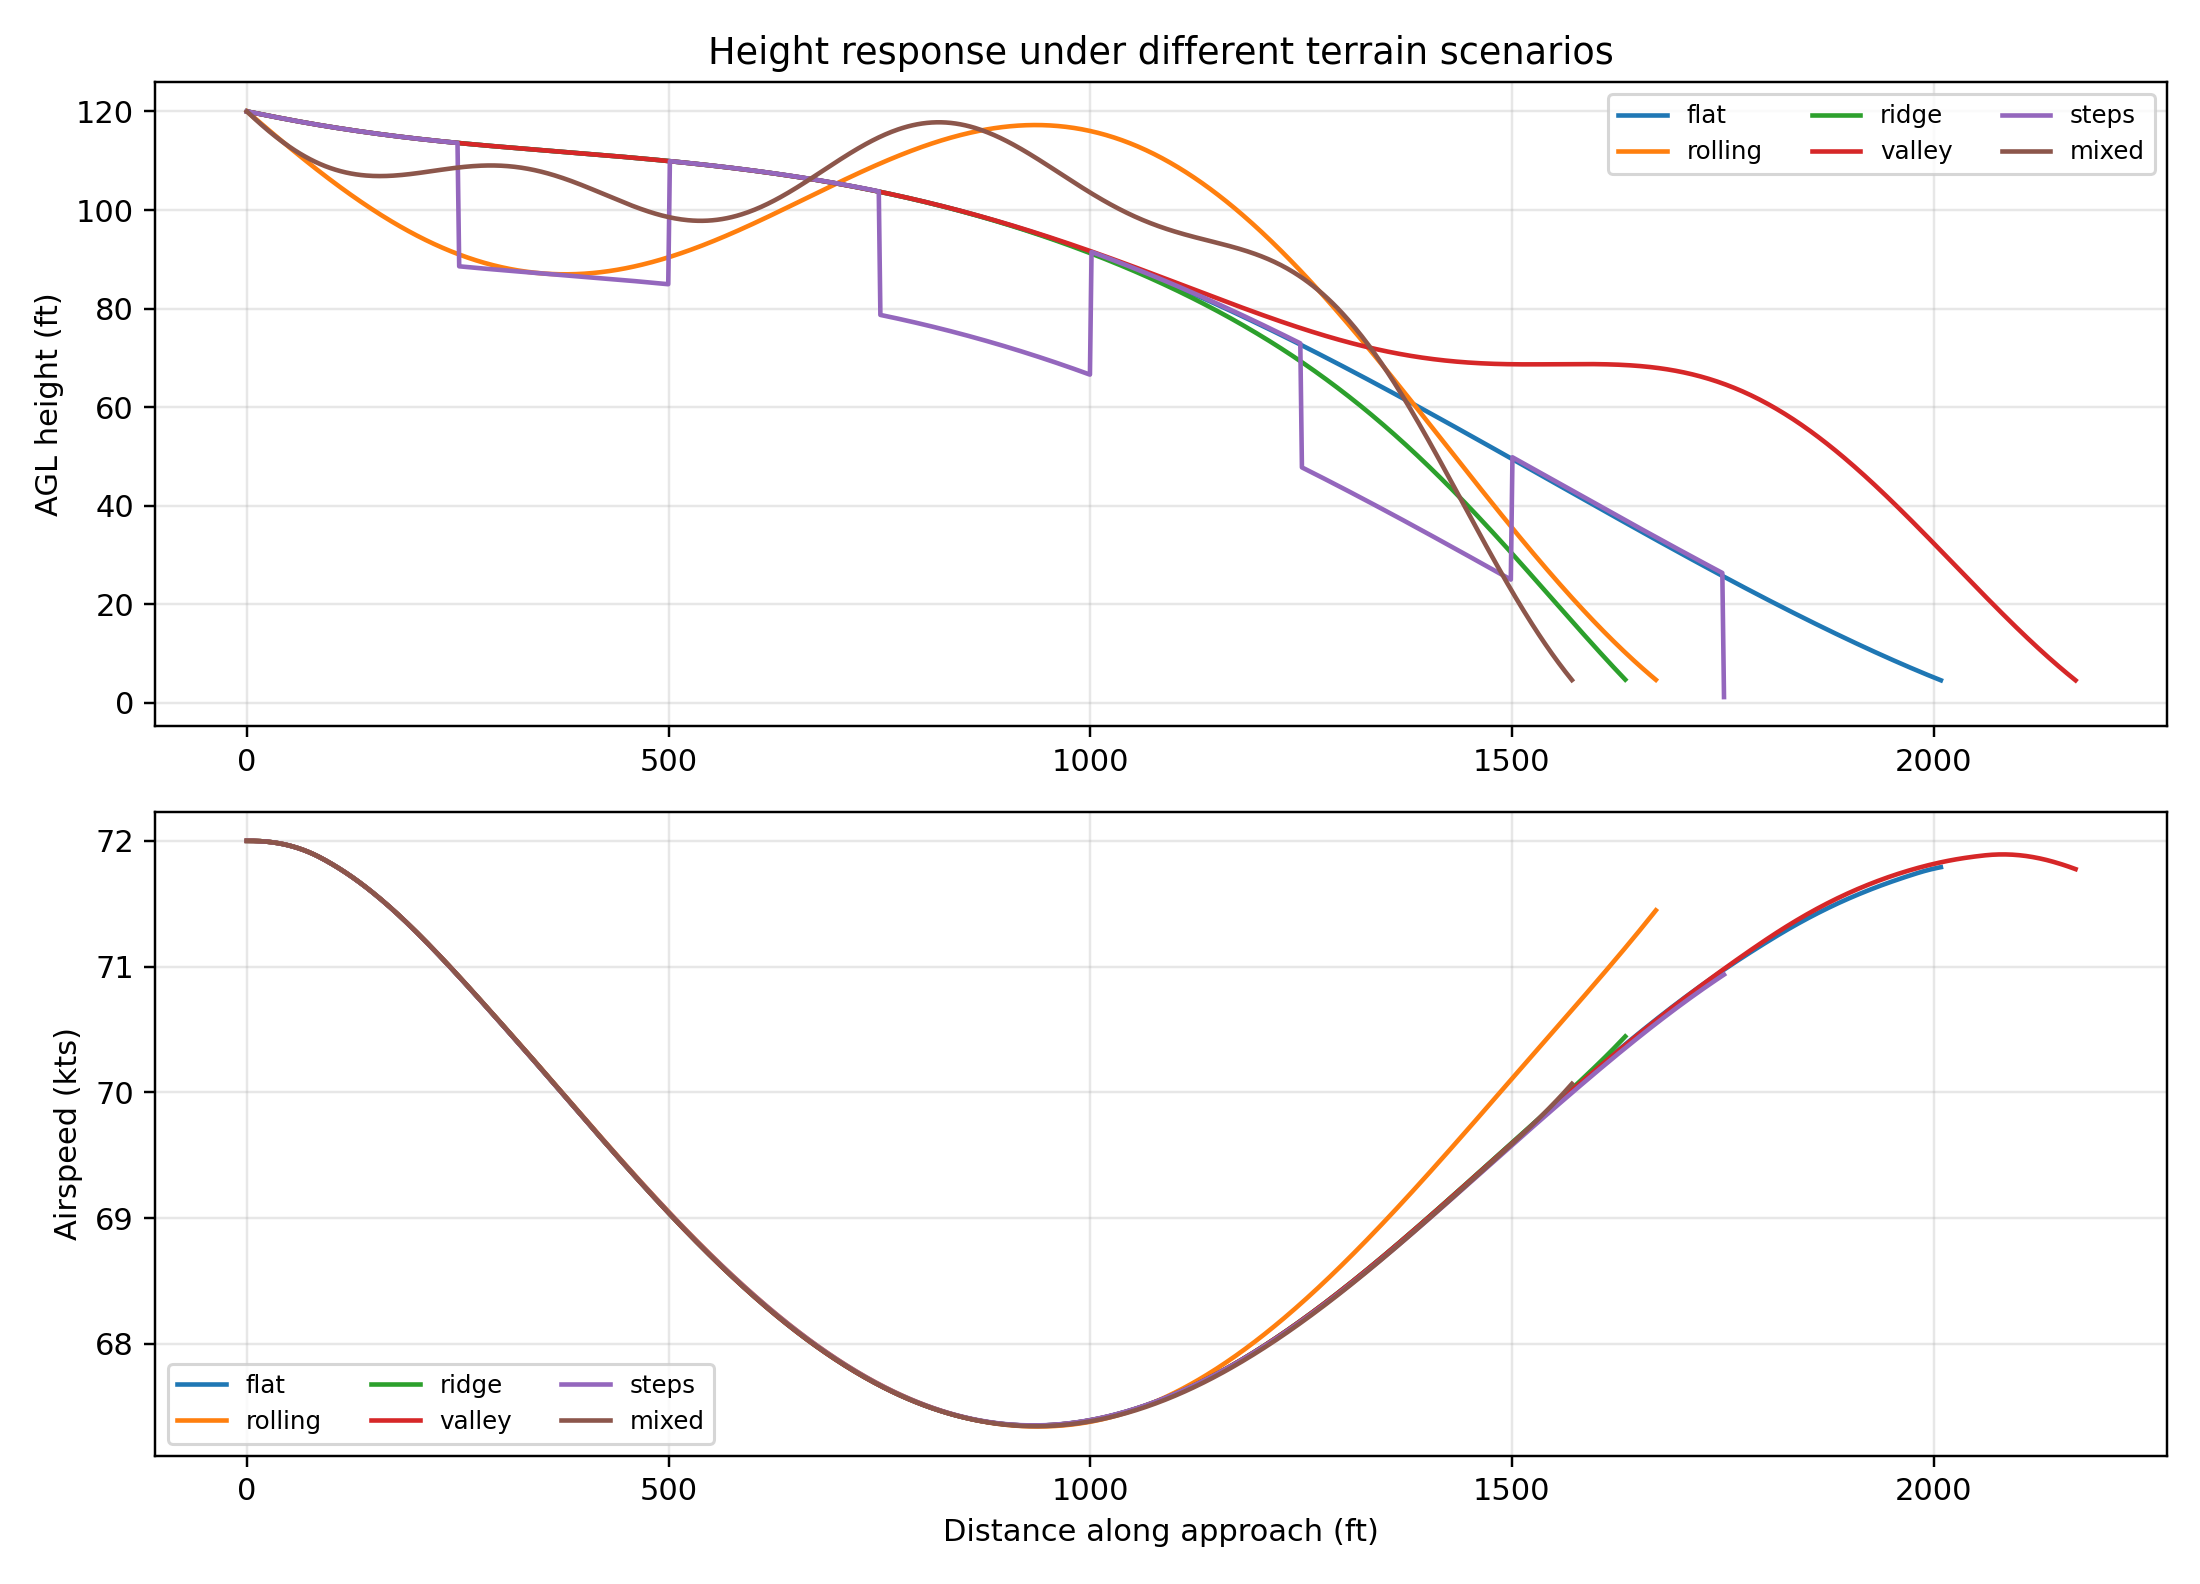
\includegraphics[width=5.45in,height=0.66\textheight,keepaspectratio]{images/image13.png}
\caption{不同地形工况下离地高度与空速响应对比}
\label{fig:5-1}
\end{figure}

就速度保持规律而言，在各个工况下飞行器末段的速度，整体上都被控制在了安全范围之内，这表明系统大体上能够达成速度约束这项任务。不过不同地形条件下速度调节的难度存在差异。在平坦地形、谷地地形工况里，速度变化相对比较平稳顺利，末段速度保持的效果比较理想，在起伏地形和山脊地形工况中，因为要同时兼顾高度修正、姿态调整，速度波动有一定程度的增加，在阶跃地形工况中，尽管速度没有显著超出界限，然而由于近地阶段高度变化更为突然，速度控制与姿态控制之间协调的压力明显更大。

依据姿态变化规律来分析，在平坦地形工况里，俯仰角、滚转角的变化幅度是最小的，这意味着系统于标准着陆条件下能够维持较好的纵横向稳定性。在起伏地形与山脊地形工况当中，飞行器为了持续对下滑状态、跑道对准进行修正，俯仰角跟滚转角的波动会更加明显。在谷地地形工况中，俯仰角整体来说比较平顺，然而滚转角呈现出一定的偏转特征，这表明其横向稳定性受到了地形的影响。在阶跃地形工况中，姿态修正最为频繁，这体现出系统需要在较短时间内同时兼顾高度、速度、方向的控制。可以看出，地形越是复杂，着陆末段状态变化就越敏感，系统对于操纵辅助、风险提示的需求也就越强。

\section{不利工况与较优工况识别}

按照之前所建立的评价指标与判据，能够对五类工况的优劣予以识别。从末段AGL、末段速度、俯仰角、滚转角、控制过程平顺性这几个方面进行综合考量，平坦地形工况的整体表现最为出色，能够当作较优工况。在该工况下，飞行器沿着预定的轨迹稳定下降，末段离地高度大概是4.60
ft，末段速度约为71.80
kts，俯仰角、滚转角都处于相对稳定的水平，这表明系统在标准环境中具备较好的收敛性与稳定性。

图~\ref{fig:5-2}从最大侧偏、最大下沉率和告警占比三个维度对比了不同地形工况下的系统表现，可作为安全性与稳定性的综合评价依据。

\begin{figure}[H]
\centering
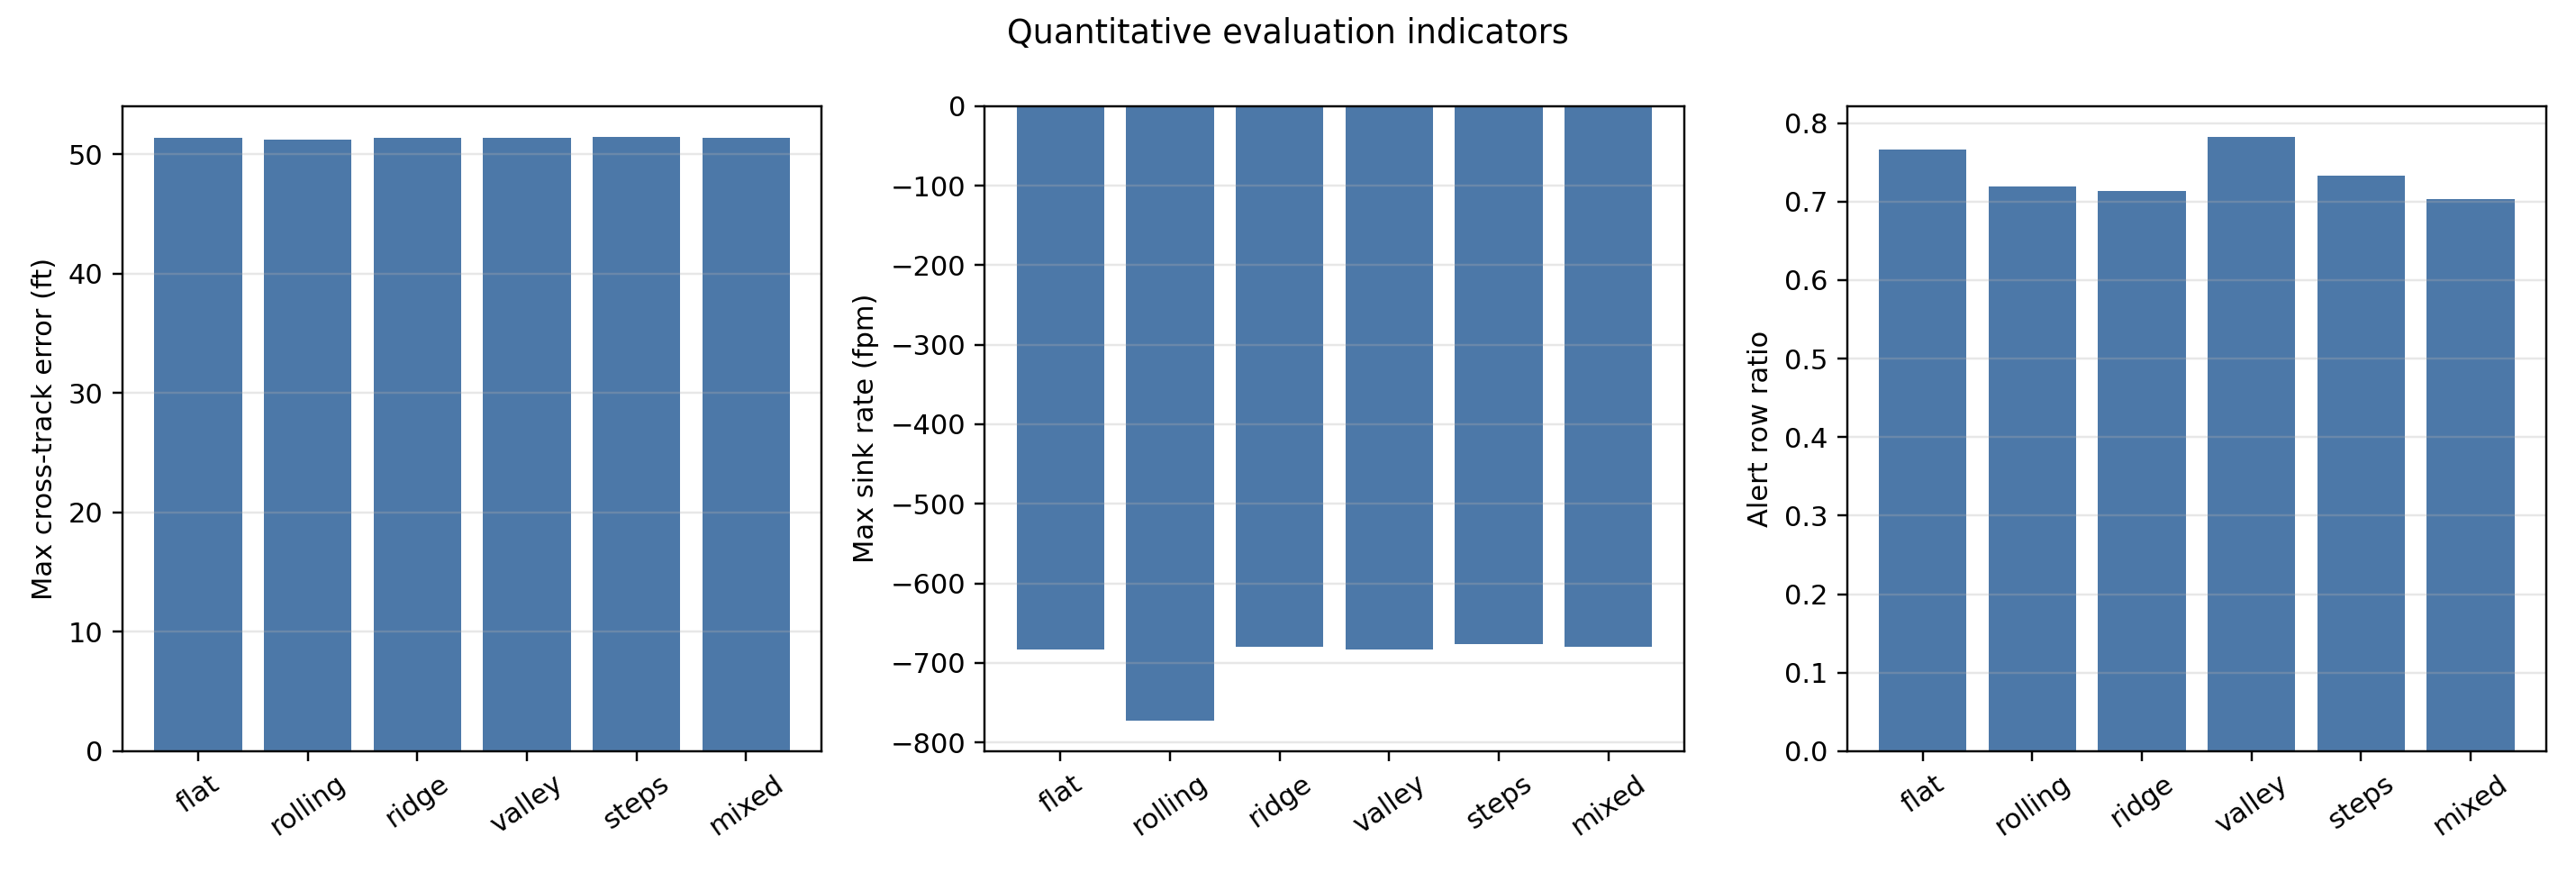
\includegraphics[width=0.92\linewidth,height=0.66\textheight,keepaspectratio]{images/image14.png}
\caption{多地形工况下关键评价指标对比}
\label{fig:5-2}
\end{figure}

谷地地形工况的仿真总时长比较长，不过末段速度保持的效果不错，末段离地高度和平坦地形相近，俯仰角的变化也比较小，故而总体性能比较理想，可当作次优工况。该工况的主要特点是前段控制裕度大，系统能较去进行轨迹修正，所以末段状态总体比较平顺。

起伏地形工况、山脊地形工况能够被归结为偏不利的工况类型。在起伏地形工况之中，俯仰角、滚转角所产生的变化幅度相对较大，这意味着系统需要持续地对处于连续变化状态的地面高程作出响应。而在山脊地形工况下，鉴于地形在接近区域呈现出快速抬升的趋势，飞行器相对离地高度的减小速度更为迅速，倘若控制修正稍微出现滞后的情况，便极易对拉平质量产生影响。所以，这两种工况尽管并未导致明显的失稳现象发生，却已然比较暴露出系统在复杂环境下所存在的薄弱环节。

在各种工况中，阶跃地形工况可被判定为最为不利的工况。其最为突出的一个特征在于，末段AGL仅仅约为1.20
ft，这一数值明显低于其他工况的相应数值，这说明地形发生突变后，近地阶段的控制调整空间被极大幅度地压缩了。该工况末段滚转角的绝对值相对比较大，这表明横向姿态保持的难度也随之增大了。虽说速度并没有出现严重越界的情况，但是高度突变对于操纵者判断拉平时机、接地窗口造成了比较明显的干扰。所以，在后续进行人机交互强化策略分析、系统优化的时候，阶跃地形工况是需要重点予以关注的对象。

\section{典型工况机理解释}

平坦地形工况能够呈现出比较优异的工况表现，其主要缘由在于地面高程基本维持恒定状态，飞行器海拔高度与相对离地高度之间的关系清晰明了且简单易懂，系统能够依据预先设定的下滑角、目标速度、阶段切换规则实现稳定运行，操纵者对于末段接地时机的判断也更易于与系统提示达成一致，如此一来整体控制便最容易趋向收敛。

为能更详细地说明控制器在典型工况下的行为表现，图~\ref{fig:5-3}展示出俯仰角、滚转角、升降舵、油门指令同步变化的情况，以此来呈现控制器完成下滑、修正、接地这一系列连贯动作的方式。比如，在下滑阶段，油门和升降舵共同作用去维持目标空速、下滑角，在拉平阶段，升降舵上偏的指令会使飞行器抬头，从而减小下沉率。

\begin{figure}[H]
\centering
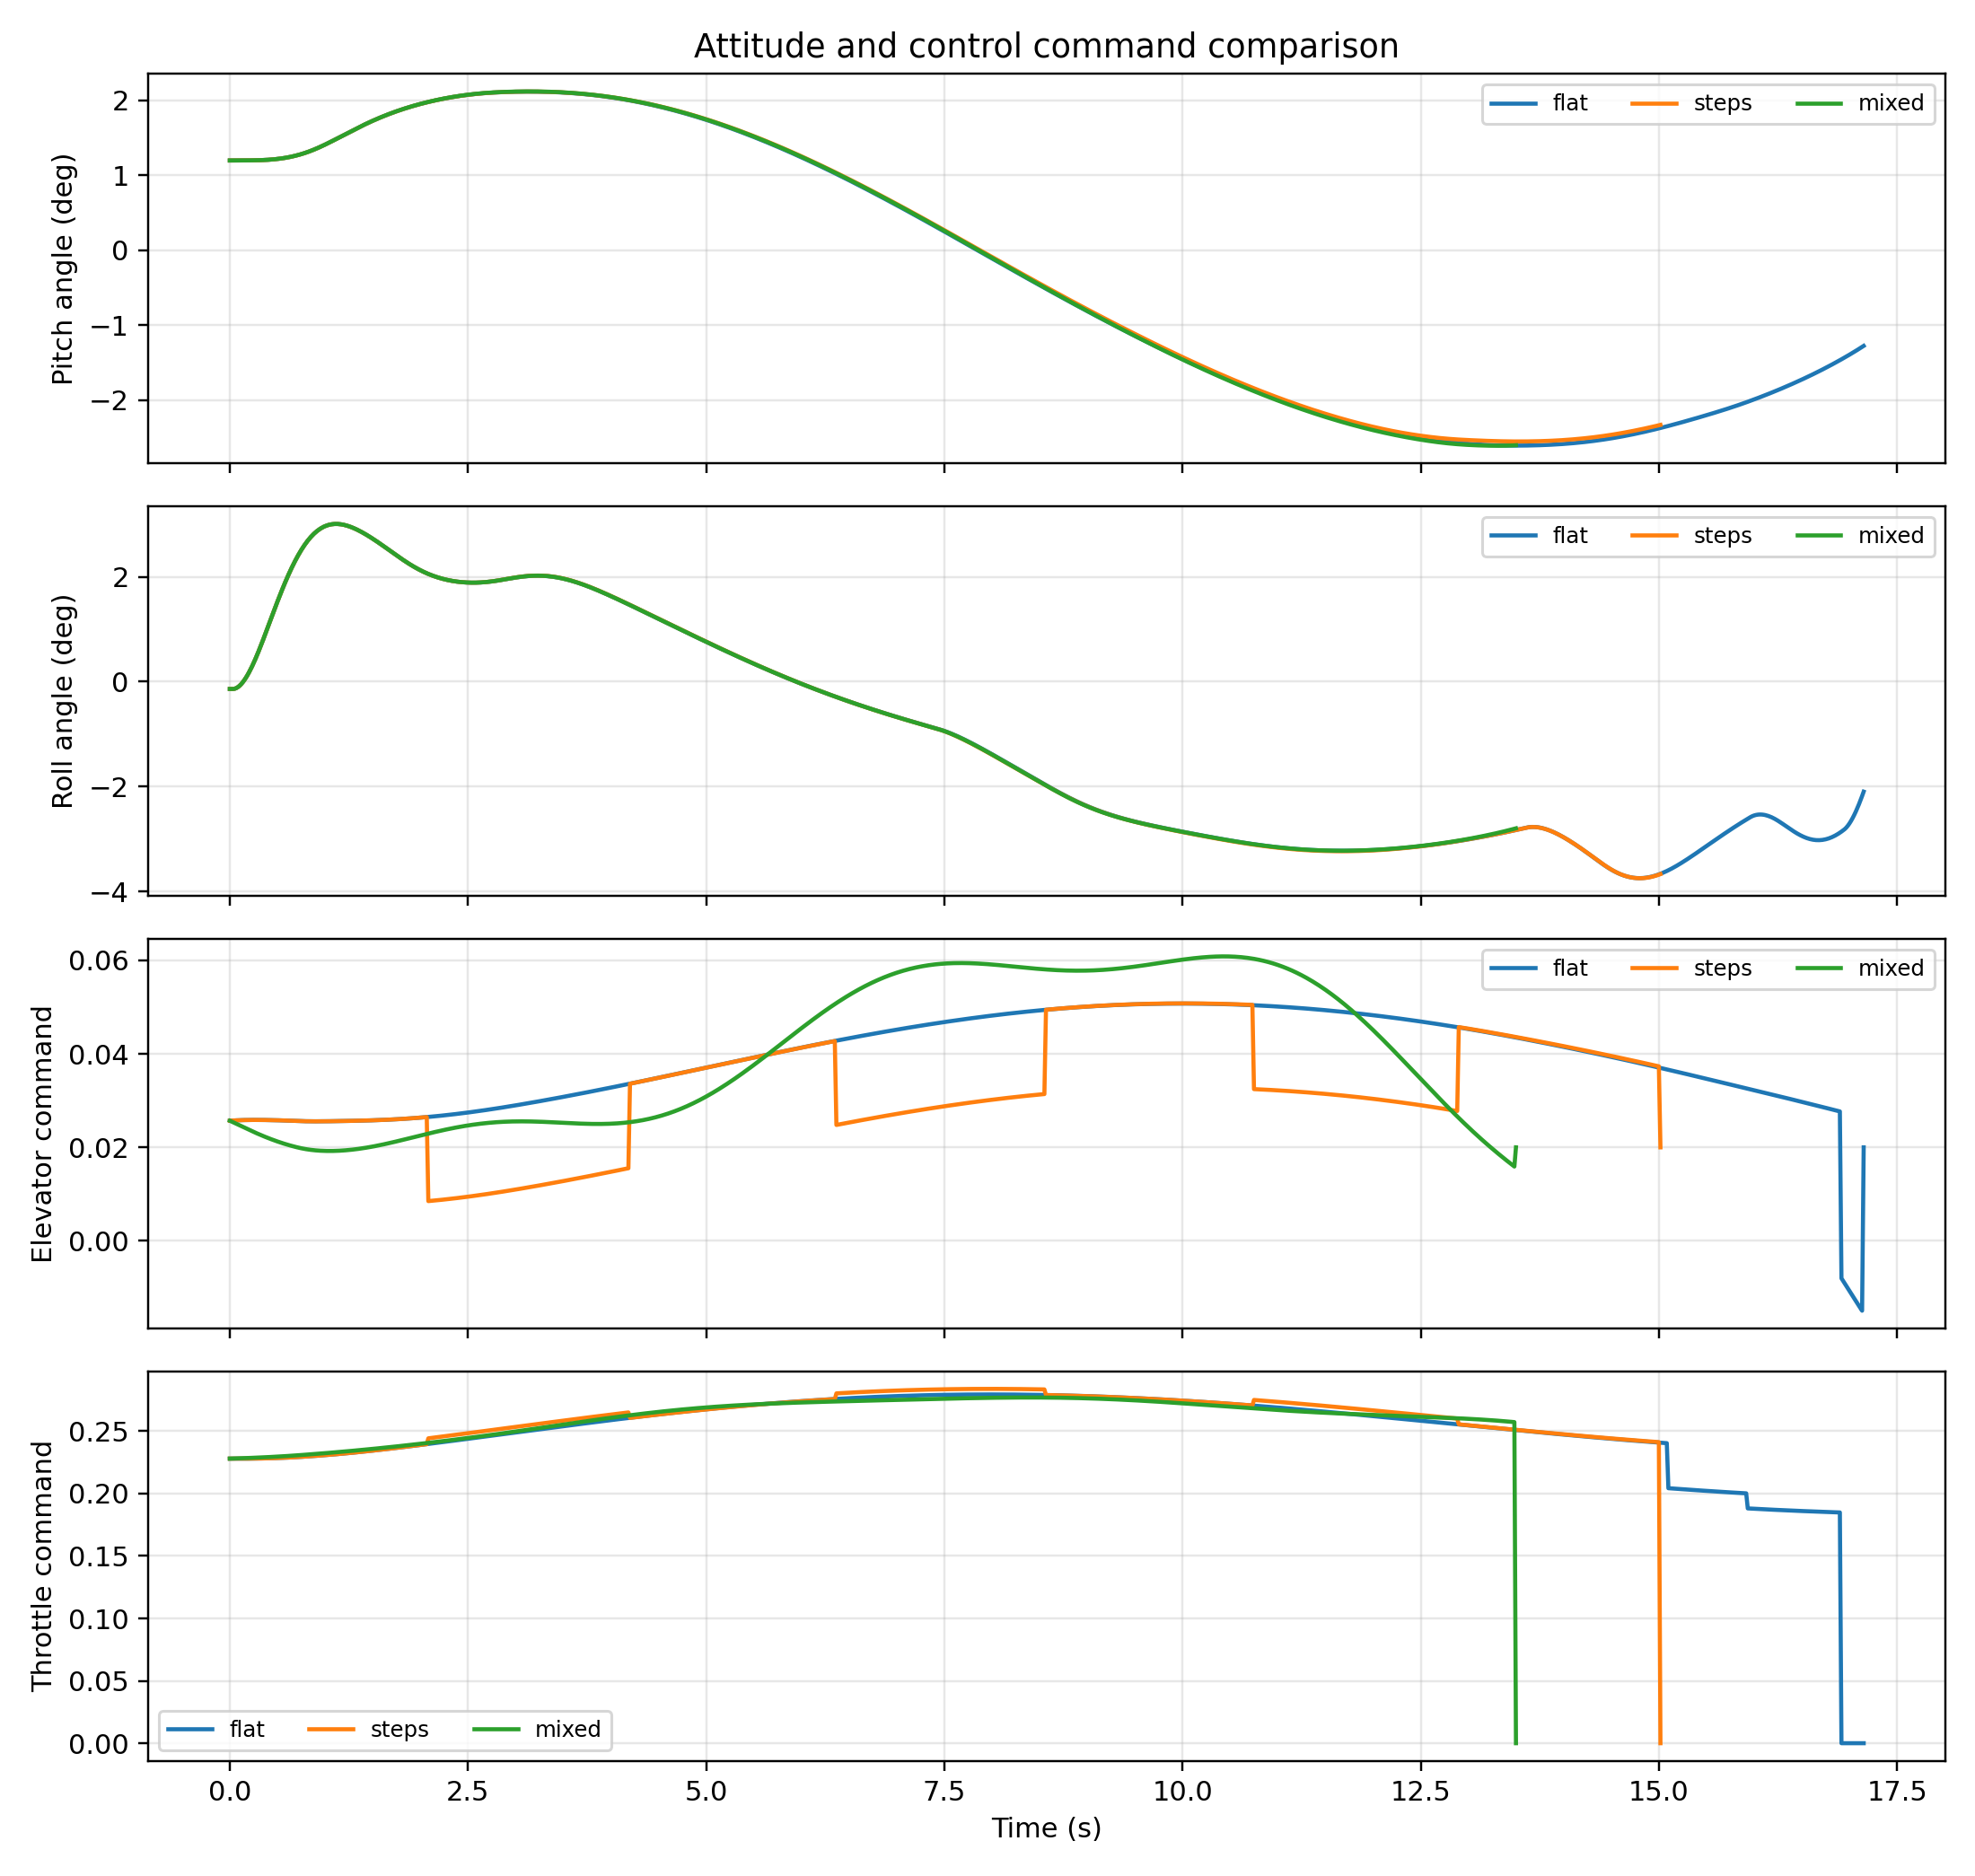
\includegraphics[width=3.99in,height=0.66\textheight,keepaspectratio]{images/image15.png}
\caption{典型工况下姿态角与控制指令变化}
\label{fig:5-3}
\end{figure}

山脊地形工况所存在的问题主要是因为在接近跑道之前地面高程迅速上升。飞行器海拔高度尽管依旧平稳下降，然而其相对离地高度会在较短时间内急剧减小，使得系统必须更早地完成下沉率抑制、姿态修正。要是修正速度偏慢，就容易导致拉平不足的情况发生，要是修正过度，又有可能致使姿态波动有所增加。山脊地形工况体现出系统对于地形的快速变化比较敏感。

阶跃地形工况被认为是最不利的，其根本缘由是地面高程的不连续变化使得飞行器相对离地高度突然降低。对于操纵者来说这种情况会压缩反应时间，而对于控制系统而言则会加大阶段识别、边界判断、接地时机控制的难度。也就是说这种工况并非只是纵向控制困难，而是高度判断、姿态控制、接地窗口识别同时变得困难。所以在复杂地形特别是阶跃型地形条件下，仅仅依靠基础控制律难以充分确保着陆品质，还需要借助更清晰的状态提示、风险告警、约束保护来提高系统鲁棒性。

综合来看，通过多工况分析能够发现，平坦地形能够当作系统的基准参考，谷地地形整体呈现出较好的状况，起伏、山脊、阶跃地形则更能够体现系统在复杂环境下的风险特性。其中，阶跃地形属于最为典型的不利工况，应当作为后续人机交互强化设计、系统优化时重点分析的对象。

%!TEX root = ../hutbthesis_main.tex

\chapter{人机交互强化策略分析与系统优化}

\section{风险识别与告警分级策略}

固定翼飞行器着陆阶段的风险并非在接地瞬间才会出现，而是在进近、拉平、接地区域逐渐累积起来。所以人机交互强化首先需要解决的问题便是及时识别关键风险，再通过分级告警的方式去提醒操纵者。从前面的仿真结果能够知道，复杂地形、下沉率偏大、侧偏增加还有姿态波动加剧，这些都会提高着陆风险，特别是在山脊地形和阶跃地形当中，这种风险更为显著。

本文的观点是，风险识别应当围绕着飞行速度、下沉率、俯仰角、滚转角、侧偏量、航向误差、跑道相对位置等状态量来进行。其中，速度能够主要反映出是否存在失速或者过快接地的风险，下沉率主要反映的是接地冲击风险，俯仰角与滚转角主要反映姿态超限风险，侧偏量、航向误差反映的是跑道对准状态。为了提高提示的效果，本文把告警划分成了三级：一级是提示级，意思是状态偏离了目标但还没有接近边界，二级是警示级，意味着关键参数接近限制范围，三级是危险级，表明系统已经接近或者进入了明显不利窗口，在这个时候应该触发保护逻辑或者复飞/中止机制。吕健玮等人在无人机短距着陆控制技术研究里指出，短距着陆条件下控制窗口更小，所以风险识别必须提前进行。这一思路同样适用于本文的固定翼飞行器着陆控制系统。

\begin{figure}[H]
\centering
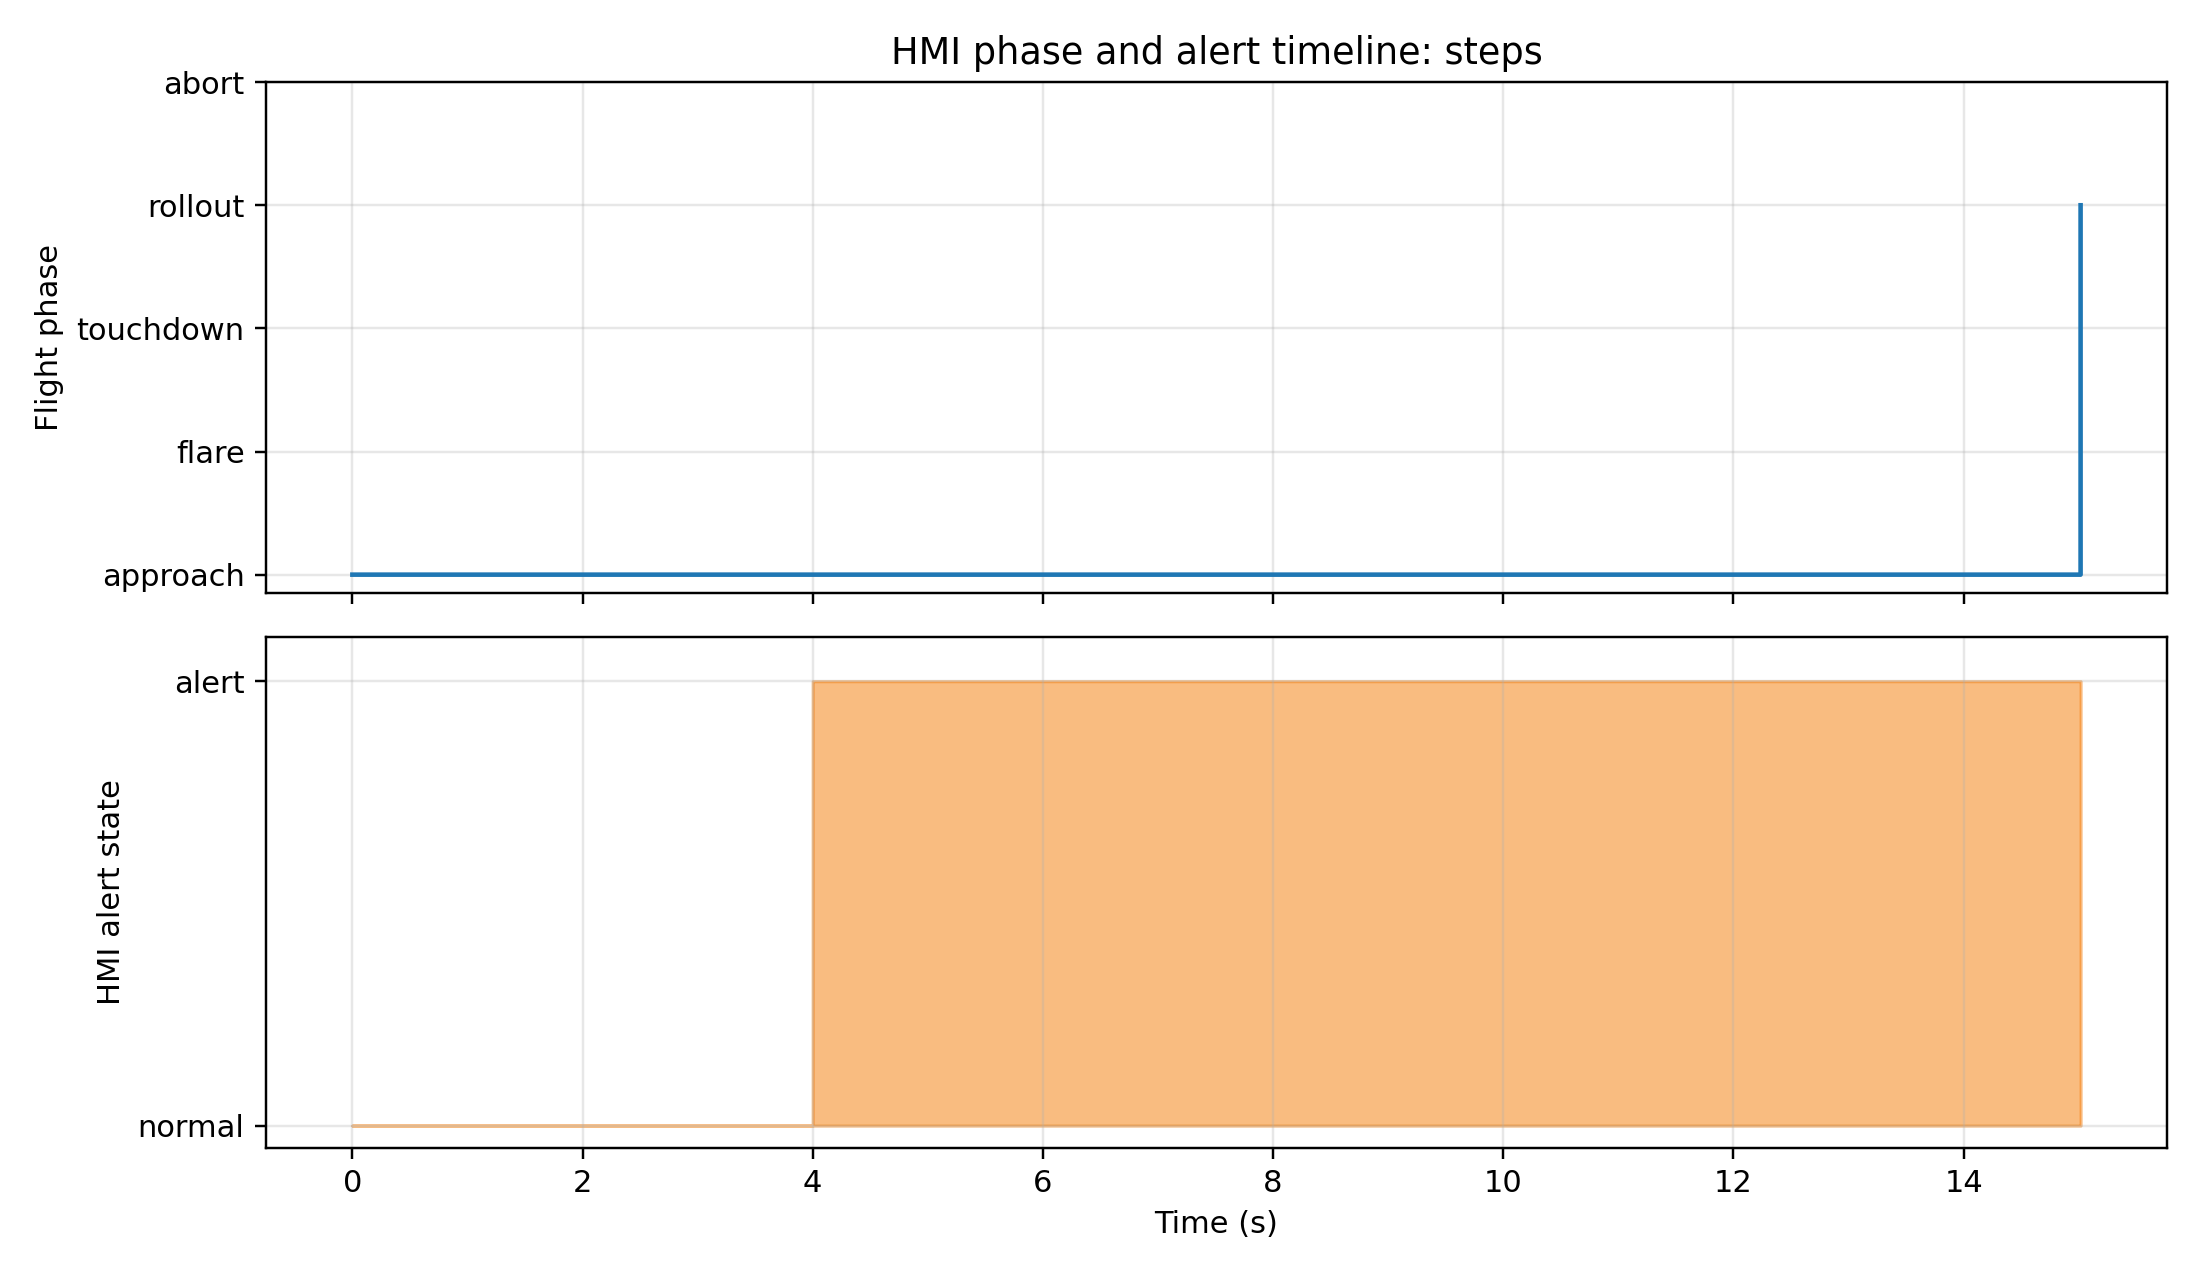
\includegraphics[width=0.92\linewidth,height=0.66\textheight,keepaspectratio]{images/image16.png}
\caption{阶跃地形工况下飞行阶段与HMI告警状态变化}
\label{fig:6-1}
\end{figure}

图~\ref{fig:6-1}以阶跃地形工况为例，展示了飞行阶段与HMI告警状态随进近过程的变化。可以看到，告警状态随进近、捕获和接地阶段动态变化，充分体现了HMI对风险状态的实时提示能力。

\section{状态提示、操纵辅助与约束控制设计}

在人机交互强化设计当中，风险识别仅仅只是基础内容，而真正对改善着陆品质起到关键作用的是状态提示、操纵辅助、约束控制这三者的协同配合。此篇论文依据现有的仿真平台界面、控制逻辑，把人机交互强化功能归纳为``提示---辅助---约束''这样的三层结构。第一层为状态提示层，第二层是操纵辅助层，第三层是约束控制层。这三层结构会按照由弱到强的顺序逐渐介入，如此既能保留操纵者的参与感，又能够在高风险阶段给予必要的保护。

状态提示层设计的关键在于追求``简单、直接、可理解''。因为着陆末段操纵负荷比较高，系统不应给操纵者传递过多冗余信息，而是要着重展示最关键的状态量。具体涵盖离地高度、速度、下沉率、俯仰角、滚转角、侧偏量、跑道剩余距离、目标接地点相对位置等。并且能够借助颜色变化、趋势箭头或者文字提示等形式，对``偏大''\,``偏小''\,``趋于危险''等状态予以直观呈现。例如，当下沉率不断增大时，给出``近地阶段下沉率偏大''的提示，当侧偏量迅速增大时，提示``检测到侧偏，正在修正''，当进入跑道捕获区时，提示``已进入跑道捕获区，优先保持接地稳定''。这种状态提示设计的作用，并非取代操纵者进行判断，而是减轻其在末段的信息整合负担。

操纵辅助层的关键要点是``给予方向，而非进行替代''。当飞行器状态快要接近风险边界，然而还未进入危险状态的时候，系统需要向操纵者输出相关建议信息，像是建议增大或者减小俯仰修正、提醒保持中心线、提示优先控制下沉率等情况。对于末段着陆来讲，这种辅助有着特别重要的意义，这是因为操纵者常常会在高度快速发生变化时出现操作方面的犹豫或者过度修正。段鹏在无人机短距着陆纵向控制技术研究里表明，短距着陆纵向控制的关键之处在于接地前速度和下沉率的协同约束。这一结论意味着，在人机交互强化的过程中，操纵辅助不应该是模棱两可的``注意安全''，而应该尽可能围绕纵向控制核心变量给出清晰明确的建议。

为验证不同控制模式的效果，本文在阶跃地形这一不利工况下，对比了正常模式与保守模式。从图~\ref{fig:6-2}可以看出，保守模式通过更高的速度安全裕度和襟翼约束，使接地阶段高度余量由正常模式的约1.20
ft提高到约4.68 ft，这体现了人机交互强化策略对风险工况的辅助作用。

\begin{figure}[H]
\centering
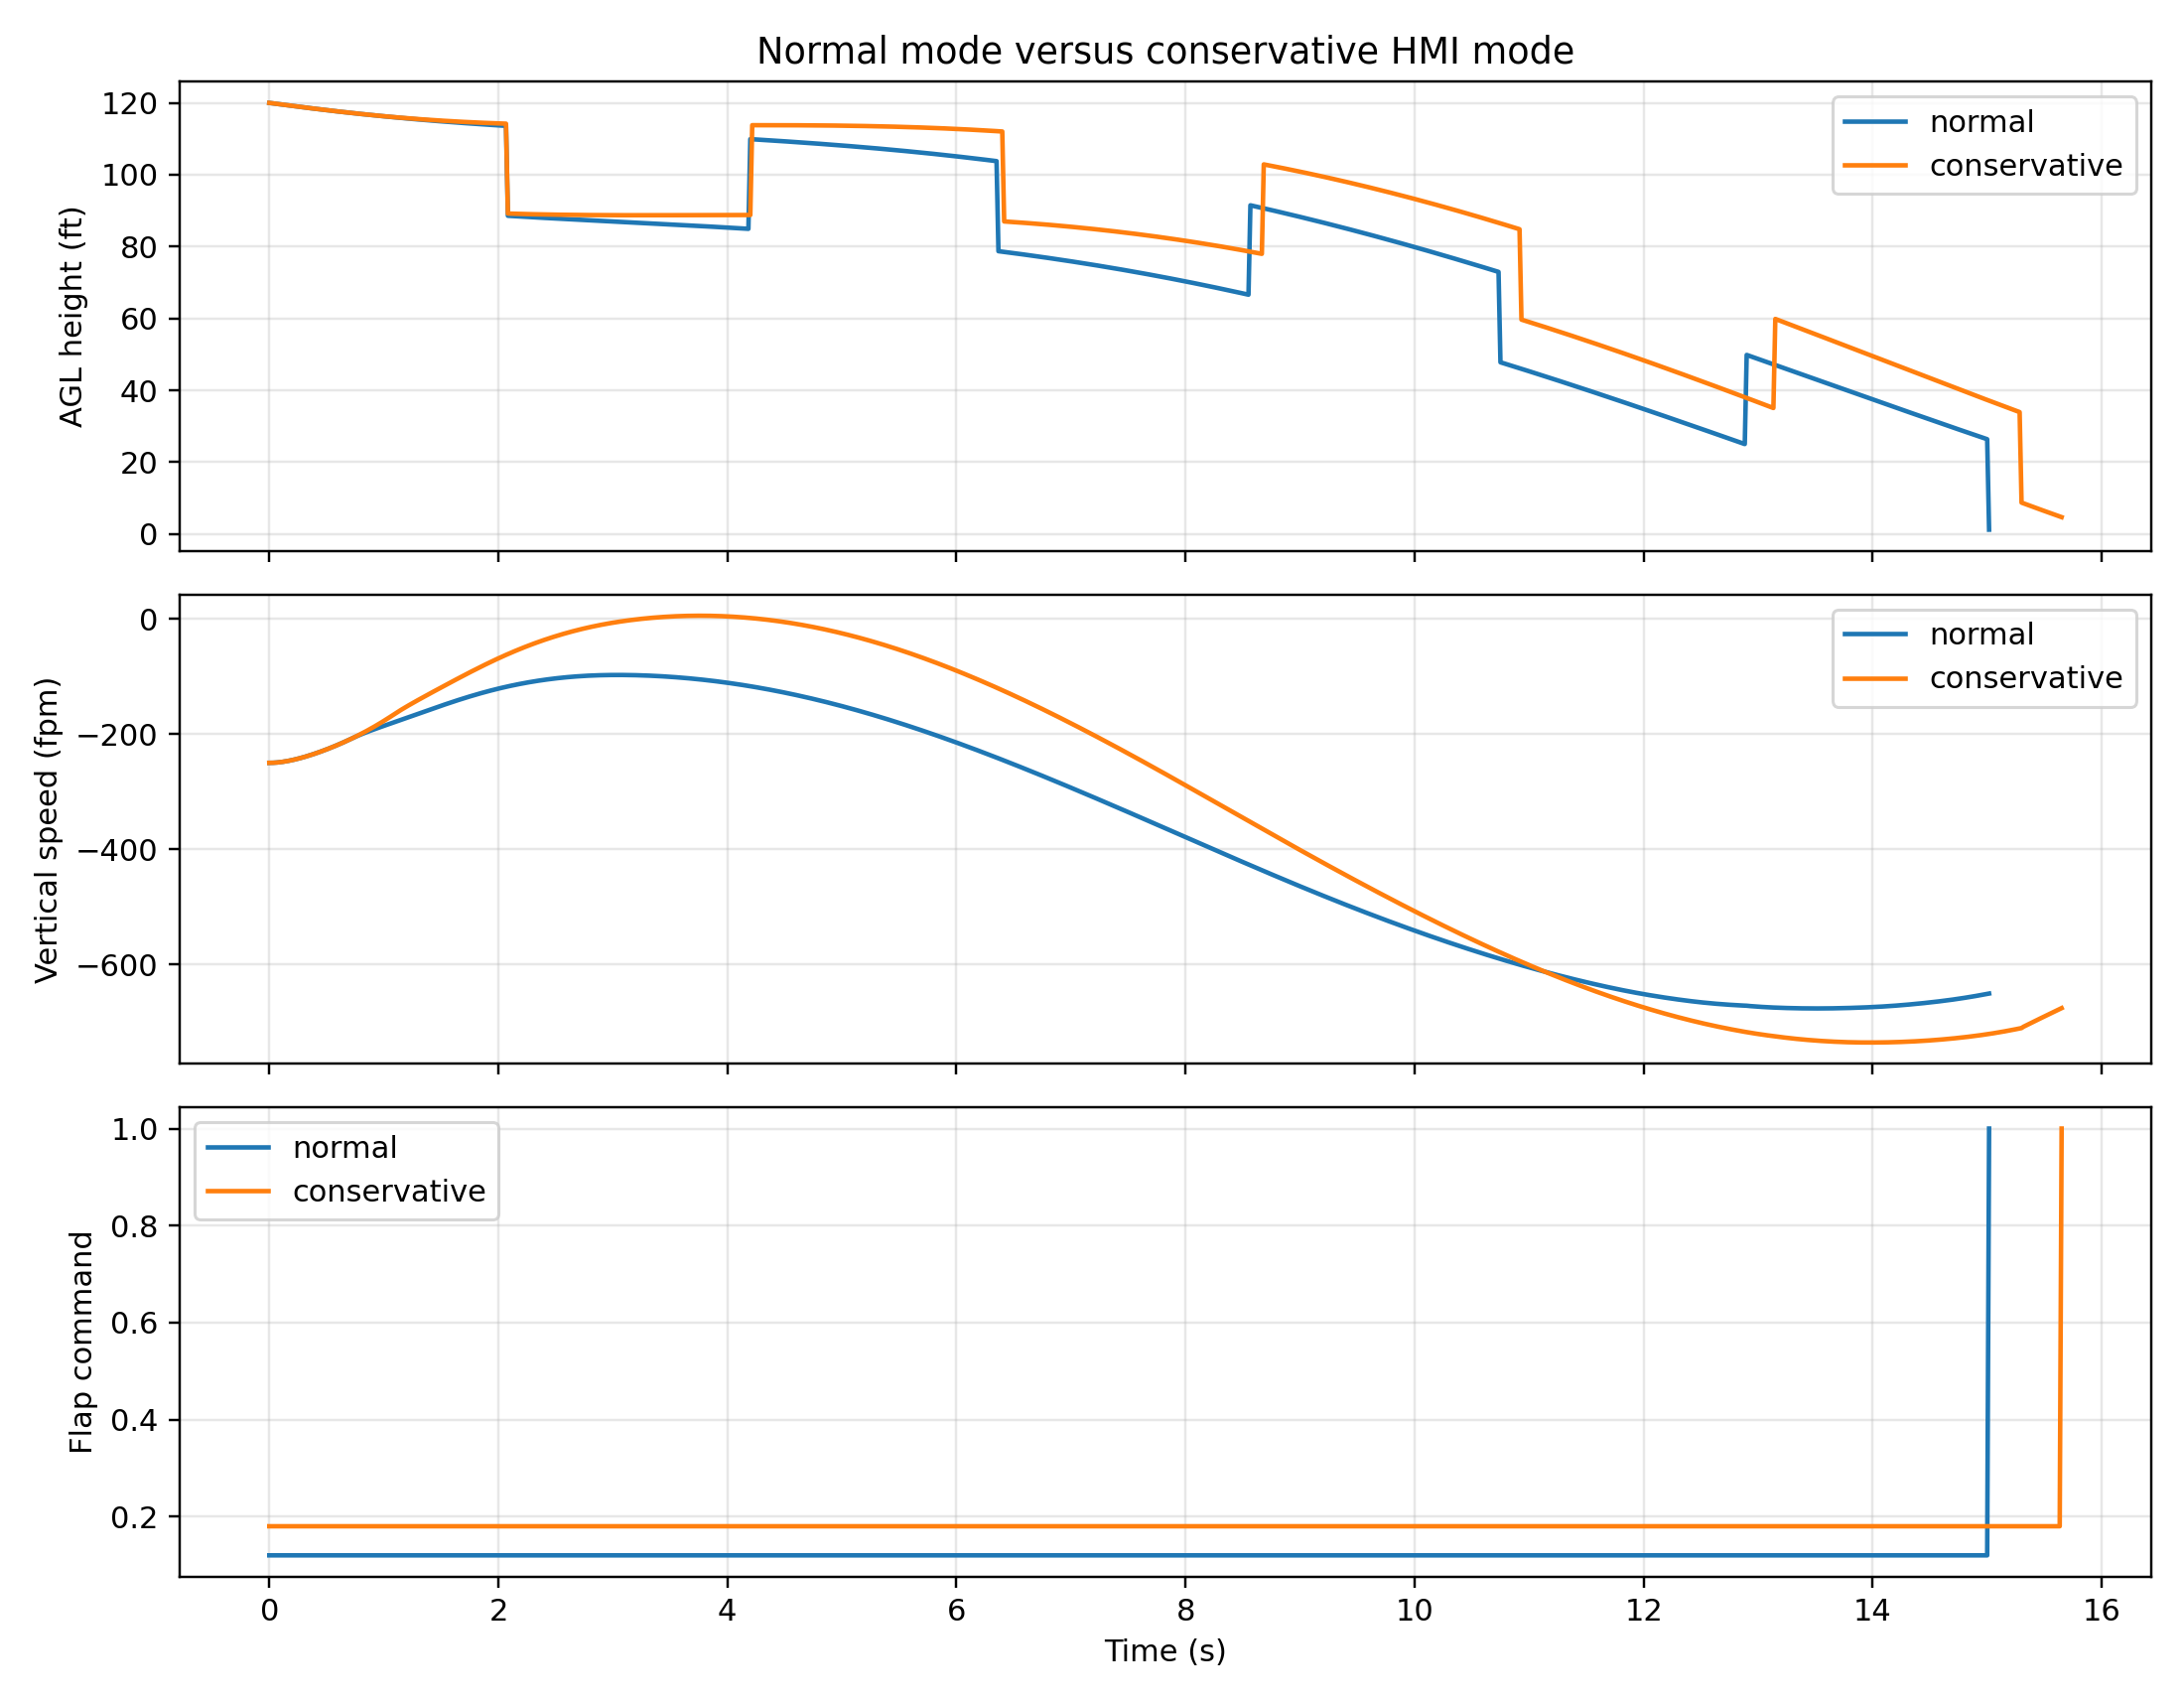
\includegraphics[width=5.19in,height=0.66\textheight,keepaspectratio]{images/image17.png}
\caption{正常模式与保守模式下着陆响应对比}
\label{fig:6-2}
\end{figure}

约束控制层为人机交互强化的最后一道保障。当根据前文风险识别判定飞行器已逼近危险边界，或者操纵输入有可能致使姿态快速恶化之际，系统需要针对部分输入实施限幅、整形或者强制约束。举例而言，在近地阶段对副翼和方向舵的过大修正予以限制，以此防止横向姿态突变，当速度过低时提高油门下限，避免进入危险低速区，在下沉率严重超出限定值时，触发更强的拉平控制或者复飞保护。约束控制的目的并非完全接管操纵，而是在关键窗口防止系统进入不可恢复状态。所以可以看出，状态提示、操纵辅助、约束控制并非相互孤立的三项功能，而是依据风险程度逐级增强的统一策略。

\section{关键参数敏感性分析}

为了弄清楚究竟哪些参数对于着陆品质、交互强化效果有着最为显著的影响，在本研究当中，需要针对关键参数进行敏感性分析工作。结合前文所提及的模型、工况结果，本研究挑选出目标速度、下沉率阈值、拉平高度、跑道捕获距离、侧偏约束、滚转角约束等作为敏感性分析的具体对象。之所以选择这些参数，主要是因为它们在控制逻辑里属于关键边界条件，并且与交互提示、保护动作的触发时机直接相关联。

为了能深入去分析系统对于初始状态偏差的敏感程度，本文专门建立了速度 -
侧偏二维工况矩阵，其中初始速度分别选取64、68、72、76、80
kts，初始侧偏选取 -100、-50、0、50、100
ft，地形环境设定为阶跃地形，随后引入综合风险评分来展开分析。从图6 -
3所呈现的热力图结果能够看出，低速并且侧偏较大的这种组合风险是最高的。这也就意味着速度的保持、侧向的修正乃是HMI提示最为关键重要的方面。

\begin{figure}[H]
\centering
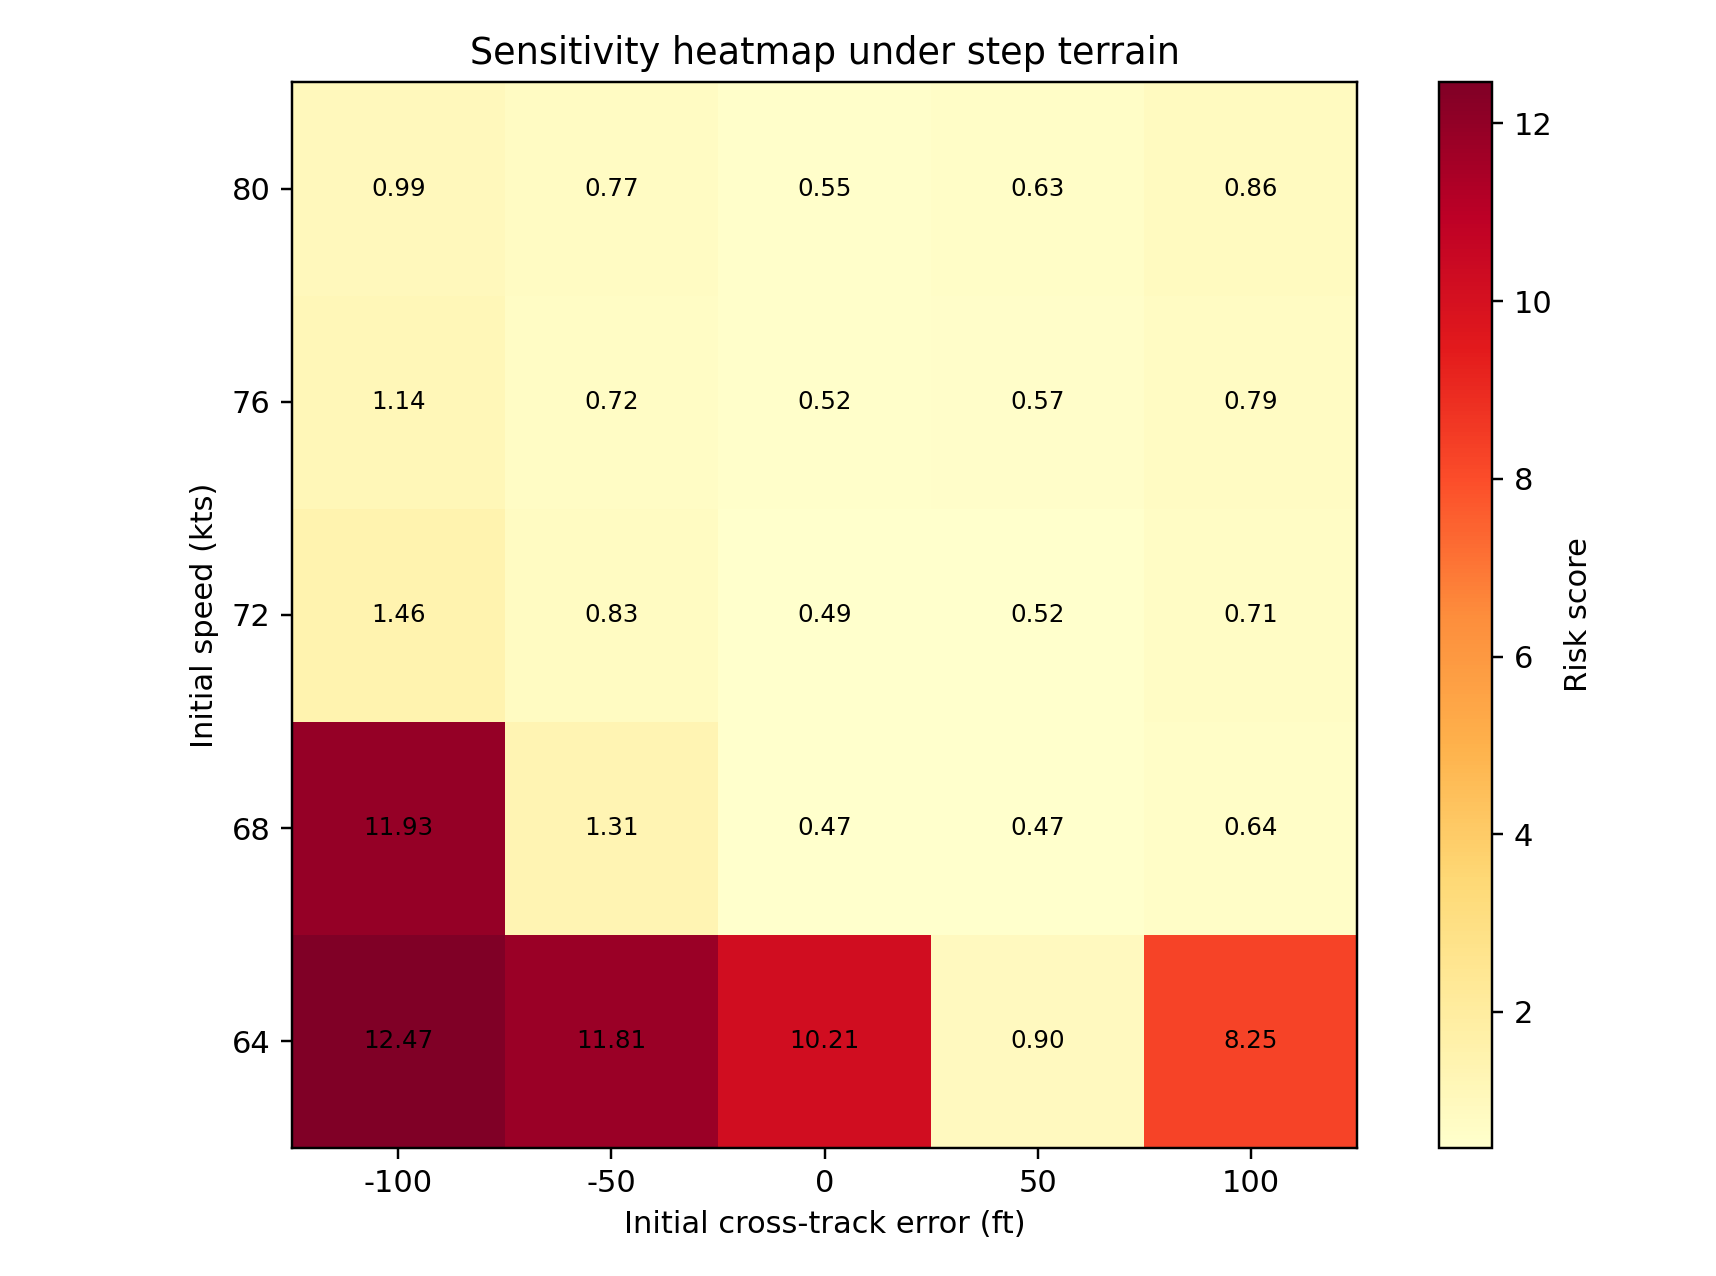
\includegraphics[width=5.43in,height=0.66\textheight,keepaspectratio]{images/image18.png}
\caption{初始速度与侧偏误差对风险评分的影响}
\label{fig:6-3}
\end{figure}

\section{改进建议与工程可实现性讨论}

借助敏感性分析能够发觉，目标速度、下沉率阈值、拉平高度对纵向品质造成的影响最为显著，而侧偏量和滚转角约束对横向稳定、跑道对准所产生的影响更为突出。这表明后续系统优化不可单纯平均地对所有参数予以调整，而应当优先围绕具备高敏感性的参数展开。喻小康在无人机概念设计与分析工具开发研究当中指出，参数化分析工具的价值体现在能够迅速识别影响系统性能的关键变量，进而提高方案迭代效率。所以，本文把敏感性分析当作连接仿真结果与工程优化的关键环节，用以给下一步参数调整、交互策略改进提供参考。

根据前文工况分析、敏感性分析的结果，本文认为针对人机交互强化的系统优化能够从四个方面着手进行。其一，对告警逻辑予以优化。需要进一步提高告警分级的针对性、可解释性，避免因提示过多而造成信息干扰，同时也要避免提示过晚进而失去干预价值。其二，优化状态显示方式。要突出离地高度、下沉率、速度、侧偏量等核心状态，以便让操纵者在末段能够迅速抓住重点，而非被大量辅助信息分散注意力。其三，优化操纵辅助策略。建议在不同的着陆阶段设置不一样的辅助优先级，比如在进近阶段优先给出轨迹与对准提示，在拉平阶段优先给出下沉率和俯仰控制提示，在接地区域优先给出稳定接地与方向保持提示。其四，优化约束控制边界。对于像拉平高度、速度下限、横向约束阈值这类高敏感参数，应当结合工况特征进行分阶段调整，而非采用固定不变的全程阈值。

为了验证约束保护策略的有效性，在本文中特意设置了大侧偏（260
ft）、大航向误差（35
deg）这样的极端工况。从图~\ref{fig:6-4}所呈现出的仿真结果能够看出，系统具备识别偏差越界的能力，并且会触发复飞保护，以此避免在不满足安全条件时还继续接地。这也就验证了约束保护层设计是很有必要的。

\begin{figure}[H]
\centering
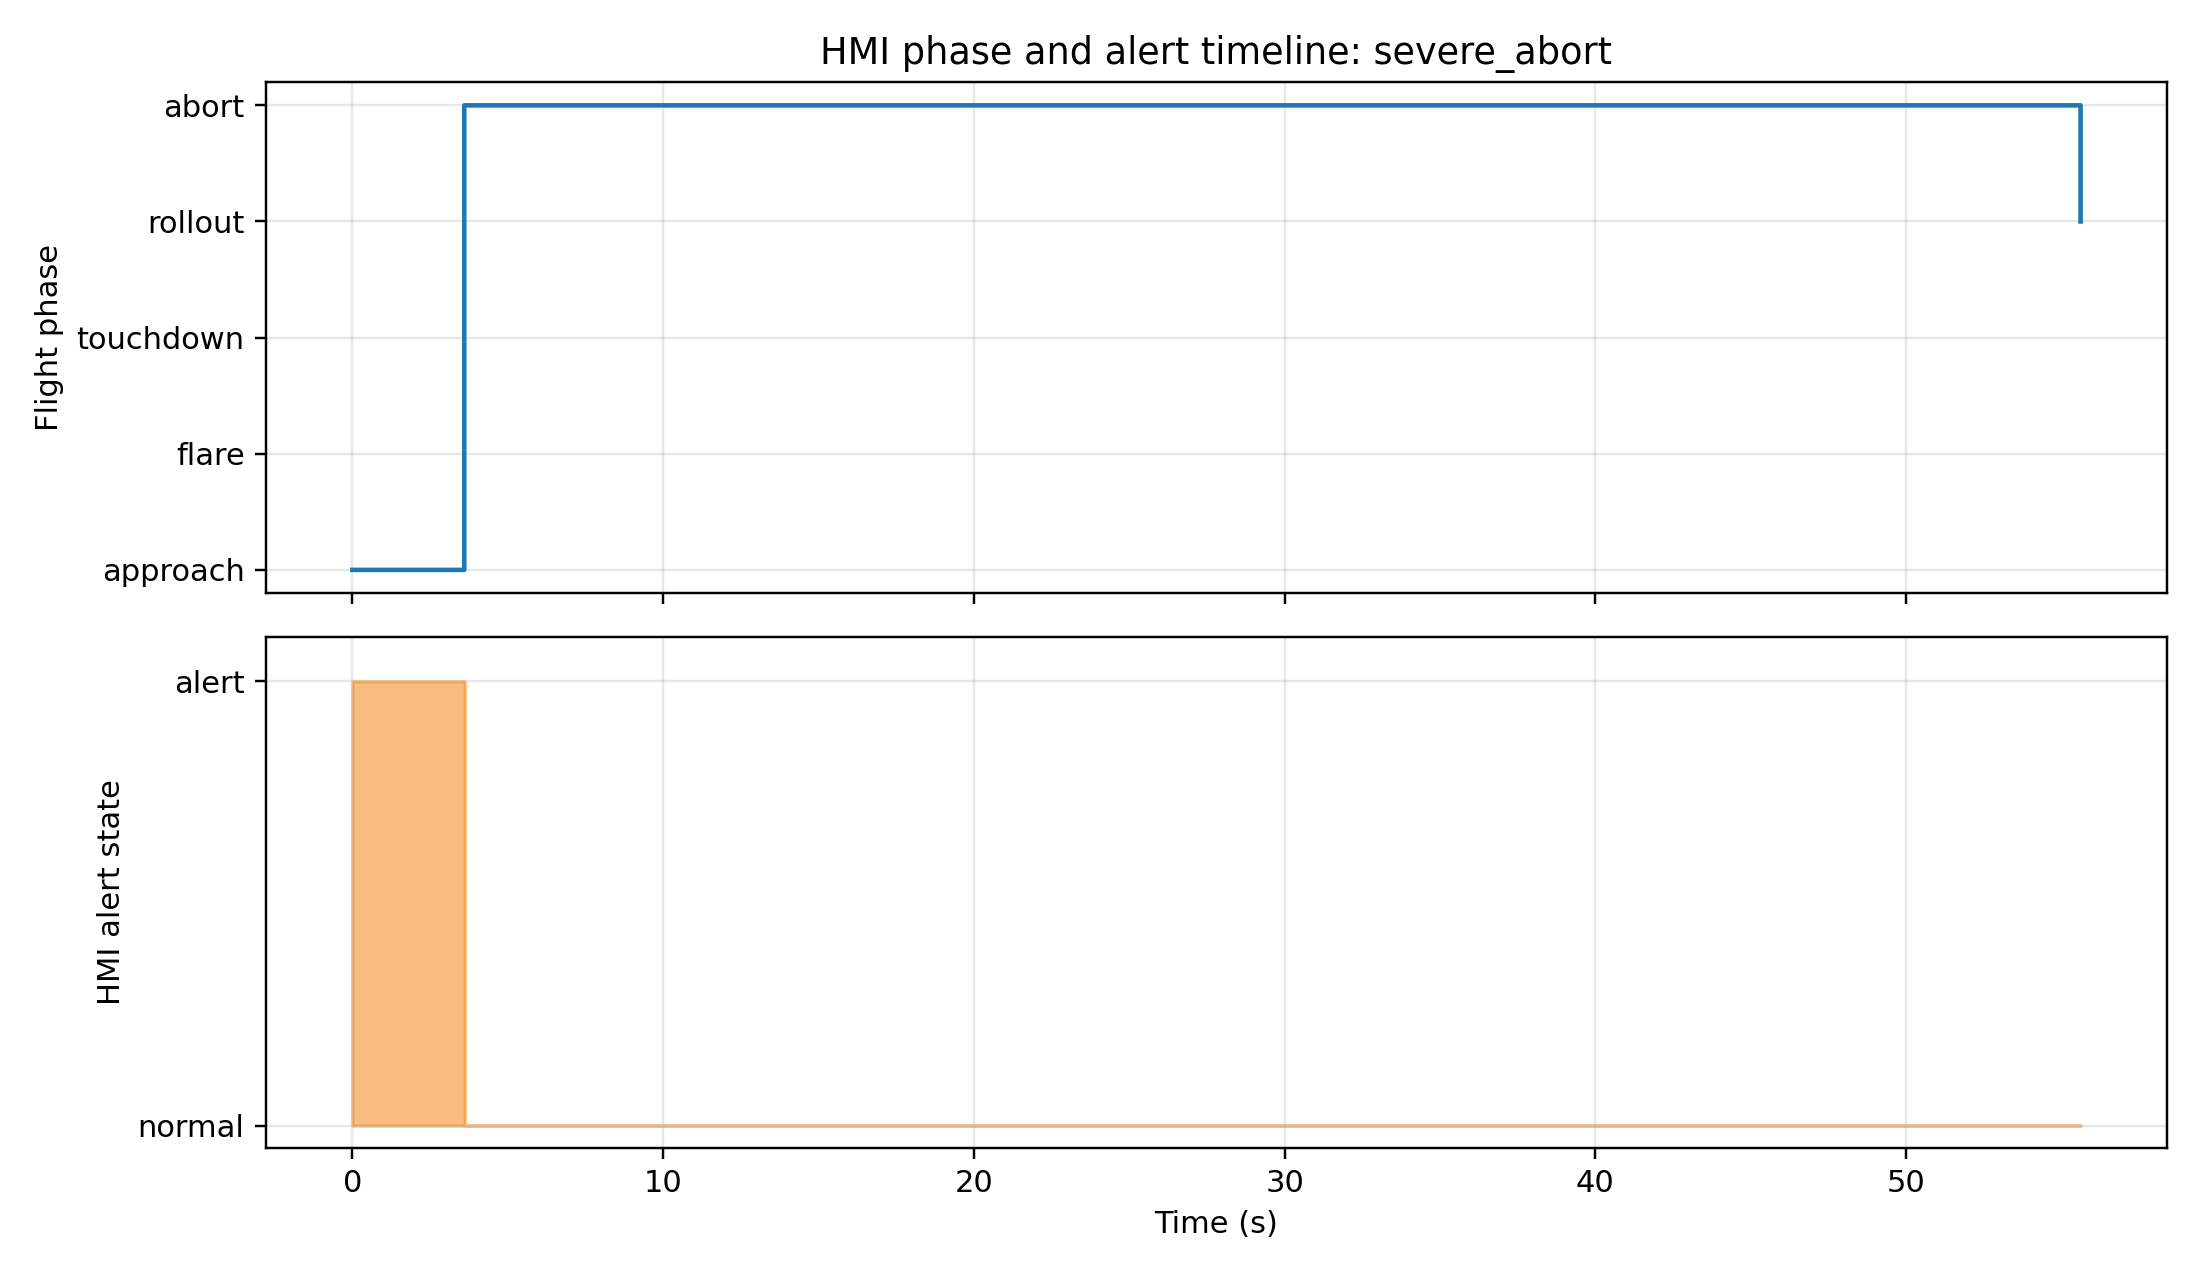
\includegraphics[width=0.92\linewidth,height=0.66\textheight,keepaspectratio]{images/image19.png}
\caption{极端偏差工况下复飞保护触发过程}
\label{fig:6-4}
\end{figure}

从工程能够实现的角度来看，本文所提出的人机交互强化策略具备良好的落地基础。第一，像速度、高度、姿态、侧偏量这些所需的关键状态量，都能够借助现有的飞控系统、导航感知系统来获取，无需额外建立太过复杂的硬件模式。第二，告警分级、状态提示、操纵辅助，本质上属于软件层的逻辑优化，可以通过飞控显示界面或者地面站界面来达成，开发成本相对而言比较低。第三，约束控制和复飞保护虽说对控制逻辑有较高要求，但在已有分阶段控制的基础上增添边界判断模块便能够实现，不需要重新建立一整套控制系统。所以，本文提出的优化策略既有理论分析的意义，也拥有一定的工程应用前景。

人机交互强化所具有的价值，并非在于替代飞行控制本身这一方面，而是在于借助``提前识别---及时提示---适度辅助---必要约束''此种方式，提高固定翼飞行器于复杂工况下的着陆稳定性、安全性。

%!TEX root = ../hutbthesis_main.tex

\chapter{结论与展望}

本文将基于人机交互强化的固定翼飞行器着陆控制系统当作研究对象，针对系统组成、需求分析、动力学模型和仿真平台建立、多工况仿真结果分析，还有人机交互强化策略设计等方面展开了研究。

研究结果表明，固定翼飞行器着陆阶段受速度、下沉率、姿态角、侧偏量以及地形环境等多种因素共同影响，是飞行全过程中控制要求较高、风险较集中的阶段。通过建立着陆控制动力学模型和仿真平台，可以较好地反映飞行器在进近、拉平和接地区域的状态变化规律。基准工况校核结果表明，所建模型具有较好的可运行性和合理性，能够满足后续工况分析需要。

多工况仿真得出的结果显示，在不同地形状况之下，飞行器着陆末段的响应呈现出显著的差别。平坦地形工况整体具备最高的稳定性，能够当作参考基线，谷地地形工况有着较好的表现，起伏地形、山脊地形会使得姿态修正频率有所增加，阶跃地形对于近地判断、接地控制产生的影响最为突出，属于最为典型的不利工况。由此能够看出，地形环境发生改变，对于固定翼飞行器着陆控制品质有着重要作用。

基于此本文形成了一种人机交互强化思路，将风险识别、状态提示、操纵辅助、约束保护整合在一起。研究显示，此策略可在一定程度上提高操纵者对于复杂工况的感知、应对能力，对于改进着陆安全性和稳定性有着积极作用。

因为研究条件、论文篇幅方面存在限制，所以本文存在一些不足之处。其一，本文主要运用仿真分析方法，对于真实飞行器复杂的气动特性、实际扰动环境的考量不够全面，后续能够结合更高保真度模型进一步优化研究。其二，本文针对起落架接地缓冲过程主要做了简化处理，后续可结合接地冲击、缓冲系统动力学展开更细致的分析。其三，本文所提出的人机交互强化策略主要在仿真平台上得到了验证，后续可结合半实物仿真或者飞行试验进一步检测其有效性。

当下，针对固定翼飞行器着陆控制系统的人机交互强化这一研究领域而言，存在着比较可观的拓展可能性。在后续的发展进程当中，可以把更为复杂的工况状况、精度更高的模型、更为完善的交互设计方式相互结合起来。通过这种结合方式，能够提高固定翼飞行器在复杂环境里的着陆安全程度，进而提高其在工程应用方面的价值。


%!TEX root = ../hutbthesis_main.tex

\clearpage
\chapter*{参考文献}
\addcontentsline{toc}{chapter}{参考文献}
\begingroup
\small
\sloppy
\begin{enumerate}
\item \hypertarget{ref:1}{}Elahi H ,Mughal R M ,Akmal W R , et al.Design and Analysis of CFRP‐Based Landing Gear for Unmanned Combat Aerial Vehicles[J].International Journal of Aerospace Engineering,2025,2025(1):7261539-7261539.
\item \hypertarget{ref:2}{}Lampropoulos K N ,Sarris E I ,Antoniou S , et al.Aerodynamic Performance of a Natural Laminar Flow Swept-Back Wing for Low-Speed UAVs Under Take Off/Landing Flight Conditions and Atmospheric Turbulence[J].Aerospace,2025,12(10):934-934.
\item \hypertarget{ref:3}{}Dinc A ,Yildiz F ,Ma J , et al.Dynamics of Oleo-Pneumatic Landing Gear Systems for Carrier-Based Unmanned Aerial Vehicles[J].Aerospace,2025,12(2):127-127.
\item \hypertarget{ref:4}{}Jinjin C ,Caijun X .Design optimisation and experimental verification of a UAV's landing gear buffer[J].International Journal of Crashworthiness,2024,29(2):320-329.
\item \hypertarget{ref:5}{}백준수,Junsoo Baek,곽준영,等.Input Signal Transformation Based Control Assistant System for UAV Moving Target Tracking and Landing Performance Improvement[J].Journal of the Korean Society for Precision Engineering,2022,39(2).
\item \hypertarget{ref:6}{}帅涛.某型起落架设计及模态分析[J].中国科技信息,2025,(11):22-24.
\item \hypertarget{ref:7}{}周著学,于萍.基于有限元分析的小型航拍无人机起落架优化设计[J].机电产品开发与创新,2024,37(06):39-44.
\item \hypertarget{ref:8}{}薛影,张超,吴星星.无人机起落架布置对起飞性能影响分析[J].中国机械,2024,(19):10-13.
\item \hypertarget{ref:9}{}罗杰,孙继勇,陈超,等.某型无人机起落架放下阶段缓冲器气液流动特性研究[J].航空工程进展,2024,15(01):118-126.
\item \hypertarget{ref:10}{}蒲雅熙.小型无人机起落架油气缓冲器气液两相阻尼特性研究[D].重庆大学,2024.
\item \hypertarget{ref:11}{}吴磊磊.某无人机油-气式缓冲器强度分析与疲劳寿命预测[D].陕西理工大学,2024.
\item \hypertarget{ref:12}{}郑振乾.无人机滑橇式起落架动力学特性分析与缓冲性能优化[D].重庆大学,2024.
\item \hypertarget{ref:13}{}李月昊.面向无人机起落架的新型惯容式缓冲系统分析与设计[D].国防科技大学,2021.
\item \hypertarget{ref:14}{}齐浩,王泽河,朱华娟,等.飞机起落架落震动力学建模及仿真分析[J].机床与液压,2021,49(08):141-146.
\item \hypertarget{ref:15}{}梅荣.某无人机起落架着陆缓冲性能优化及试验验证[D].南京航空航天大学,2019.
\item \hypertarget{ref:16}{}赵知辛,郭强,黄鸣远,等.仿竹设计在无人机起落架结构中的应用[J].机械科学与技术,2021,40(11):1798-1804.
\item \hypertarget{ref:17}{}吕健玮,黄一敏,魏硕.无人机精确着陆控制技术[J].兵工自动化,2024,43(10):79-83+96.
\item \hypertarget{ref:18}{}郑金豪.无人机精确着陆控制技术研究[D].南京航空航天大学,2023.
\item \hypertarget{ref:19}{}周乐,尹乔之,魏小辉,等.仿生四足六旋翼无人机自适应着陆性能分析[J].航空工程进展,2024,15(03):45-51+70.
\item \hypertarget{ref:20}{}吕健玮,黄一敏,魏硕.无人机短距着陆控制技术研究[J].机械制造与自动化,2024,53(02):258-265.
\item \hypertarget{ref:21}{}段鹏.无人机短距着陆纵向控制技术研究[D].南京航空航天大学,2021.
\item \hypertarget{ref:22}{}喻小康.无人机概念设计与分析工具开发[D].南京航空航天大学,2021.
\end{enumerate}
\endgroup

%!TEX root = ../hutbthesis_main.tex

\clearpage
\chapter*{附录}
\addcontentsline{toc}{chapter}{附录}


\begin{table}[H]
\centering
\caption{实验硬件配置表}
\label{tab:appendix-hardware}
\begin{tabular}{ll}
\toprule
配置项 & 参数 \\
\midrule
处理器（CPU） & Intel Core i9-14900K \\
独立显卡（GPU） & NVIDIA RTX 4090 24G \\
内存 & 64GB DDR5 6000MHz \\
固态硬盘 & 1TB NVMe M.2 \\
显示器 & 27英寸 2K 165Hz \\
\bottomrule
\end{tabular}
\end{table}

\begin{table}[H]
\centering
\caption{实验环境配置表}
\label{tab:appendix-env}
\begin{tabular}{ll}
\toprule
配置项 & 参数 \\
\midrule
操作系统 & Windows 11 \\
开发环境 & Python 3.11 \\
IDE工具 & PyCharm \\
仿真平台 & AirSim \\
\bottomrule
\end{tabular}
\end{table}

\begin{lstlisting}[style=hutbcode,language=Python,caption={着陆控制器核心代码节选},label={lst:landing-controller}]
class LandingController:

def __init__(self):

self.config = ControllerConfig()

self.mode = "normal"

self.abort_requested = False

self.abort_latch = False

self.flare_latch = False

self.landing_commit_latch = False

self.last_phase = "approach"

self._violation_time_s = 0.0

def trigger_abort(self):

self.abort_requested = self.abort_latch = True

self.flare_latch = self.landing_commit_latch = False

def reset(self):

self.mode = "normal"

self.abort_latch = self.flare_latch = self.landing_commit_latch =
False

def compute(self, s):

cfg = self.config

h_agl = s["h_agl_ft"]

v_kts = s["vc_kts"]

vs_fpm = s["vs_fpm"]

roll_deg = s["roll_deg"]

yaw_deg = s["yaw_deg"]

wow = s["wow"]

dist_rwy = s["distance_to_runway_ft"]

cross_track = s["cross_track_ft"]

rwy_hdg = s["runway_heading_deg"]

hdg_err = self._wrap_deg(rwy_hdg - yaw_deg)

dist_td = dist_rwy - cfg.target_touchdown_past_threshold_ft
\end{lstlisting}

%!TEX root = ../hutbthesis_main.tex

\begin{acknowledgements}

本论文在指导教师的悉心指导与帮助下顺利完成。在论文选题、研究思路、框架构建、设计推进以及文本修改等过程中，导师始终给予我耐心细致的指导与严格要求，在此谨向导师致以诚挚的感谢和崇高的敬意。

感谢各位任课教师在本科阶段给予我的专业教学与启发，使我在相关理论、方法与表达能力方面打下基础，为本论文研究与设计实践提供了必要支撑。感谢学院各位老师在学习与毕业论文期间提供的帮助与支持。

感谢资料搜集、案例梳理、方案研讨及文稿撰写过程中给予我建议与帮助的同学和友人，彼此的交流扶持让我在遇到难题时能及时调整方向，也让本篇毕业论文的撰写推进更为顺畅。

格外感谢家人长久以来的理解、支持与陪伴，你们在学习和生活中给予的包容与关怀，是我坚持完成学业、顺利完成论文写作的坚实底气。

受个人学识与撰写时间限制，论文中难免存在欠缺与疏漏之处，恳请各位评审老师予以批评指正，我也会以此为新的开端，在后续的学习与工作中持续精进专业能力与综合素养。

\end{acknowledgements}


\end{document}
